% \documentclass[12pt, twocolumn]{article}
\documentclass[12pt]{article}
 
% \usepackage[left=1.5in, right=1in, top=1in, bottom=1in]{geometry} 
\usepackage[left=0.75in, right=0.75in]{geometry}
\usepackage{graphicx}
\usepackage[font=scriptsize]{caption}
\usepackage[font=scriptsize]{subcaption}
\usepackage{amsmath,amsthm,amssymb}
\usepackage{bm}
\usepackage{listings}
\usepackage{color}
\usepackage{dsfont}
\usepackage{float}
\usepackage[ruled, vlined]{algorithm2e}
\usepackage{array}
\usepackage{multirow}
\usepackage{wasysym}
\usepackage[nottoc]{tocbibind}
\usepackage[round, authoryear]{natbib}
\bibliographystyle{abbrvnat} % aer/natbib/others
\usepackage[hidelinks]{hyperref}

\newcommand{\E}{\mathbb{E}}

\DeclareMathOperator*{\argmax}{arg\,max}
\def\code#1{\texttt{#1}}

\begin{document}

\title{\bf{Risk Managed Automated ETF Trading with Reinforcement Learning and Gaussian Processes}}
\author{Wesley Yuan \\ MA Statistics, Columbia University \\ wy2371@columbia.edu}

\maketitle

\abstract{The search for profitable trading strategies has consistently driven financial research. Recent advances in reinforcement learning (RL) have made it an attractive approach for studying trading behavior. However, RL algorithms aim to maximize rewards and often ignore risk which leads to large swings in P\&L for a trading agent. We introduce the use of Gaussian Process Regression (GPR) for estimation of daily returns and the associated risk measures to externally manage risk of RL trading algorithms. These estimates are then used to size trades and avoid overly risky positions. The combination of GPR risk management with RL trading agents leads to improved risk metrics and often times increased cumulative P\&L over the backtesting period.}

\section{Introduction} \label{intro}

Trading, as decision making under uncertainty, is naturally framed as a reinforcement learning (RL) problem where an agent learns optimal behavior from interactions with its environment. Recent results in RL applications in other domains (\cite{Silver2017}, \cite{GoogleAtari}, \cite{AlphaGo}) have again raised interest in its use for optimal trading. 

Most applications of RL to the trading problem have a singular focus on maximizing discounted rewards (typically change in portfolio value called P\&L for profit and loss). While strategies produced from this method have been profitable (\cite{Deng2017}, \cite{Yang2020}), they fail to take into account the risk associated with achieving these returns. Some recent work has been done in using mean-variance portfolio allocation via RL (\cite{Wang2019}) but minimizing variance, while lowering risk, also limits upside potential. A better method would be to minimize some risk measure such as value-at-risk (VaR) or conditional value-at-risk (CVaR, also known as expected shortfall) that only limits downside potential. 

Several works have shown the efficacy of using Gaussian Process Regression (GPR) for risk measure estimation. \cite{Wilkens2019} use GPR to reprice instruments within a portfolio and use the confidence intervals derived from the posterior of trained GPR to estimate VaR and CVaR. \cite{Cakmak2020} takes a more general approach in modeling some black-box objective function as a Gaussian process and using Bayesian optimization to effectively sample from the posterior in estimating VaR and CVaR.

In another vein of research, Gaussian processes have been applied to stock trend predictions to try to estimate future price movements (\cite{Farrel2007}). These models rely on hand-crafted features such as daily open, close, high, low prices. In addition, predictive technical indicators such as moving averages (\cite{Park2007}) are added to help increase accuracy. Combining this with \cite{Cakmak2020} using single asset returns as the objective function, we obtain a method for risk measure estimation for the single-asset trading problem.

There has been some work in fully combining Gaussian processes into reinforcement learning algorithms to create fully Bayesian RL (BRL) (see \cite{Ghavamzadeh2016} for a full survey) that would allow for uncertainty (risk) measures in the RL decisions. These have provided certain theoretical guarantees of convergence of BRL algorithms and their associated regret bounds, they remain expensive or impossible to implement in practice. Many BRL algorithms require sampling from an extremely varied and flat posterior as number of possible beliefs grow exponentially with time. Further, some algorithms require querying some "oracle" to update distributions over transitions and observations which clearly do not exist in real-world settings. Therefore, our approach simply uses the GPR to augment decisions as a risk-manager for the pure RL system.

The rest of this paper is organized as follows. Section \ref{background} goes over preliminaries for risk measures, Gaussian processes, and reinforcement learning algorithms. Section \ref{methods} describes the details of our training scheme as well as the trading environment and implementation. Following that is the results in section \ref{results} that show how our GPR-augmented agent performs compared to a buy-and-hold strategy and the base RL strategy. Finally, section \ref{conclusion} discusses take-aways from our results and suggests possible extensions for future work.

\section{Background} \label{background}

\subsection{Risk Measures}

Risk measures are heavily used in financial applications for measuring exposure and determining asset reserves to comply with regulations. For the trading problem, a common way to measure risk is with the volatility or the standard deviation of returns. However, volatility is neutral of the direction of variation and while large negative deviations are bad, large positive deviations are good but instead are penalized.

Another common risk measure that does not suffer the problem of penalizing positive deviations is Value-at-Risk (VaR). Intuitively, VaR is an estimate of how much value a set of investments might lose under normal conditions. Let $P$ be the P\&L distribution of some position. The $\alpha$\% VaR of $P$ is given by the $1 - \alpha$ quantile i.e.

\begin{equation}
VaR_{\alpha}(P) = \inf\{p \in \mathbb{R} | F_P(p) > \alpha\} = F^{-1}_p(1 - \alpha)
\label{eq:var}
\end{equation}

While VaR can be viewed as the maximum loss of a position with $\alpha$ probability, it can also be viewed as the minimum loss of a position with $1 - \alpha$ probability. A natural question would then be, what is the expected loss given such a $1 - \alpha$ event? This defines the Conditional Value-at-Risk (CVaR) measure or Expected Shortfall (ES) which is given by

\begin{equation}
CVaR_{\alpha}(P) = \frac{1}{\alpha}\int_0^{\alpha}VaR_{\gamma}(P)d\gamma
\label{eq:cvar}
\end{equation}

Notice that by taking the expected value within some region rather than focusing on quantiles, CVaR is more sensitive to the shape of the tail of the distribution and could provide more accurate measures of risk associated with a position. Both of these measures are considered in choosing the set of actions taken by the GP-adjusted model as described in section \ref{methods}.

\subsection{Gaussian Processes}

Gaussian processes (GP) were chosen because they provide a fast and simple way of estimating mean returns and their associated uncertainties from historical data that can be updated sequentially. First, Gaussian processes are non-parametric models and therefore are able to fit to any data we choose to train on. Furthermore, recent improvements in efficiency and the availability of high-quality implementations that are compatible with current leading deep learning frameworks make them increasingly attractive for many regression tasks.

A Gaussian process is a collection of random variables, any finite number of which have a joint Gaussian distribution (\cite{Rasmussen2006}) and is completely determined by a mean and covariance (kernel) function, $m(\bm{x}), k(\bm{x},\bm{x}')$, respectively. These two are given by

\begin{align}
m(\bm{x}) & = \E[f(\bm{x})] \\
k(\bm{x},\bm{x}') & = \E[(f(\bm{x}) - m(\bm{x}))(f(\bm{x}') - m(\bm{x}'))]
\label{eq:gp eq}
\end{align}

for some process $f$ and thus we define

\begin{equation}
f(x) \sim \mathcal{GP}(m(x), k(x,x'))
\label{eq:gp def}
\end{equation}

In practice, $m(\bm{x})$ is often just $0$ as data can be de-meaned in processing to achieve this zero-mean result. Thus, the model is mostly determined by the choice of kernel function and corresponding parameters. Many possible kernel functions exist but the most commonly used ones are the squared exponential, the rational quadratic, periodic, and Matern kernels. Further, these kernels can be combined through addition and multiplication to create more complicated kernels that are able to capture more of the underlying structure in the training data. Choosing appropriate kernels and its associated hyperparameters is a rich area of research and is beyond the scope of this project. For the purposes of this project, we use a simple scaled rbf kernel and train via gradient descent using the \href{https://github.com/cornellius-gp/gpytorch}{\code{gpytorch}} package (\cite{gardner2018gpytorch}).

Given this choice of kernel function, we then have that for random vectors $\bm{y}$ drawn from a GP trained on input points $X$ has the following distribution

\begin{equation}
\bm{y} \sim \mathcal{N}(\bm{0}, K(X,X))
\label{eq:gp dist}
\end{equation}

where $K$ is the covariance matrix whose $i,j$-th element is $k(\bm{x}_i, \bm{x}_j)$. The joint distribution of training outputs $\bm{y}$ and test outputs $\bm{y_*}$ is then 

\begin{equation}
\begin{bmatrix}
\bm{y} \\
\bm{y_*} \\
\end{bmatrix}
\sim \mathcal{N}\left(
\bm{0},
\begin{bmatrix}
K(X,X) & K(X,X_*) \\
K(X_*,X) & K(X_*,X_*) 
\end{bmatrix}
\right)
\label{eq:gp post}
\end{equation}

Updates to the GP can be made by conditioning the above joint Gaussian prior on new observations to obtain our posterior distributions 

% For two-column format
% \begin{equation}
% \begin{split}
% \bm{y_*}| & X_*,X,\bm{y} \sim \mathcal{N}(K(X_*,X)K(X,X)^{-1}\bm{y}, \\
% & K(X_*,X_*) - K(X_*,X)K(X,X)^{-1}K(X,X_*))
% \end{split}
% \end{equation}

% For single-column format
\begin{equation}
\begin{split}
\bm{y_*}|X_*,X,\bm{y} \sim \mathcal{N}( & K(X_*,X)K(X,X)^{-1}\bm{y}, \\
& K(X_*,X_*) - K(X_*,X)K(X,X)^{-1}K(X,X_*))
\end{split}
\end{equation}

This posterior is the distribution from which we sample from to estimate returns and their associated uncertainties. Further, analytical values for the confidence interval of the multivariate Gaussian are obtained as thresholds for calculating CVaR from the generated samples.

\subsection{Reinforcement Learning}

Reinforcement learning is a method for solving multi-period optimal control problems by finding an optimal mapping from states to actions. The environment is modeled using a Markov decision process (MDP) that changes stochastically in response to agent actions. An agent trains through experience (trial and error) that is used to improve the agent's approximation of the action-value function of the multi-period optimal control problem. Agents in any time step $t$ act to maximize expected discounted reward defined as

\begin{equation}
G_t = R_{t+1} + \gamma R_{t+2} + \gamma^2 R_{t+3} + ...
\label{eq:discounted reward}
\end{equation}

where $R_t$ is the reward received at time $t$ and $\gamma \in [0,1]$ is a known discount rate. Having $\gamma < 1$ allows for an infinite time horizon by ensuring convergence of the sum defined by Equation \ref{eq:discounted reward}.

To maximize this reward, an agent will follow some policy $\pi$ that maps current state $s_t$ to an action $a_t$ that produces greatest expected value. An optimal policy $\pi^*$ is defined such that the following is true

\begin{equation}
V_{\pi^*}(s) \geq V_{\pi}(s)\ \forall \pi
\label{eq:optimal policy}
\end{equation}

In layman's terms, the value of being in state $s$ following $\pi^*$ as least as good as being in state $s$ and following any other policy $\pi$. There are various approaches to achieve $\pi^*$ that can be broadly categorized into variations of the following: (1) critic-only which estimates state-value functions (value iteration), (2) actor-only which learns a policy directly using action-value functions (policy iteration) and (3) actor-critic which utilizes two agents, one that learns the value function and another that learns the policy directly. This section covers relevant algorithms that were tested for this project which include: Deep Q-Learning, Deep Deterministic Policy Gradient (DDPG), Proximal Policy Optimization (PPO), and Advantage Actor Critic (A2C). For a more comprehensive survey of methods in reinforcement learning see \cite{SuttonBarto}.

The following standard notations are used in the rest of this section:

\begin{itemize}
  \item $\mathcal{S}$ and $\mathcal{A}$ are the set of states and actions in an MDP, respectively
  \item $V(s)$ denotes the value of state $s$
  \item $Q(s,a)$ denotes the value of taking action $a$ in state $s$
  \item $A(s,a)$ denotes the potential additional value of taking an action $a$ in state $s$ (i.e. $Q(s,a)$ normalized with respect to $V(s)$)
  \item $r$ denotes a stochastic reward and is a function of $s$ and $a$
  \item $R$ is the actual reward received taking action $a$ in state $s$
  \item $\mathcal{L}$ is the objective function for some algorithm
  \item $\theta, \phi$ are sets of parameters that characterize a given model
\end{itemize}

Subscripts (when present) represent the time-index. Superscripts represent the policy being followed after the immediate step.

\subsubsection{Critic-Only}

Critic-only methods determine the optimal policy by estimating the value function of the MDP being modeled. That is, the model attempts to estimate either the value of being in a given state or the value of taking an action in a given state. The optimal policy is then taking the argmax over possible actions in states. Algorithms in this class include Value Iteration, Policy Iteration, and Q-Learning, among several others. These methods are typically off-policy which means they can be trained from stored sample transitions through a method called batched experience replay. In this way, these algorithms efficiently use all transitions they experience in training. \\

\textbf{Deep Q-Learning:} First, let us consider the standard Q-learning algorithm or Temporal Difference (TD) learning algorithm. The algorithm is as follows

\medskip

\begin{minipage}{0.95\linewidth}
\begin{algorithm}[H]
  \SetAlgoLined
  \caption{Q-Learning}
  \textbf{Input:} Sequence of $\{\alpha_t\}_{t=1}^{\infty}$ (learning rates) \\
  Initialize $Q_0(a,s) = 0\ \forall (s,a)$ \\
  \For{$t = 1,2,...$}{
    \For{$(s,a) \in \mathcal{S} \times \mathcal{A}$}{
      Sample state $s_{t+1}, R_t \sim \mathbb{P}(\cdot|s,a)$ \\
      $Q_t(s,a) = (1 - \alpha_t)Q_{t-1}(s,a) + \alpha_t(R_t + \gamma V_{t-1}(s'_t))$ \\
    }
    \For{$s\in\mathcal{S}$}{
      $V_t(s) = \max_aQ_t(s,a)$ \\
    }
    $\pi_t(s) = \argmax_{a}Q_t(s,a)$
  }
  \KwResult{$\pi^*(s)$ that is an $\epsilon$-optimal mapping of states to actions}
  \label{algo:TD}
\end{algorithm}
\end{minipage}

\medskip

Q-learning can be seen as an online version of value iteration where instead of recalculating a Q-value estimate at every time step, the current estimate is updated with newly sampled information. Note that $V_{t-1} = \max_aQ_{t-1}(s_{t+1}, a)$, the update rule for $Q$ is then

\begin{equation}
Q_{t+1}(s,a) = Q_t(s,a) + \alpha_t\left(R_t + \gamma\max_aQ_{t-1}(s_{t+1},a) - Q_t(s,a)\right)
\end{equation}

The final Q-value estimate can be seen as a weighted-average of estimates from every time-step. By the update rule, this estimate is heavily dependent on the learning rates $\alpha_t$ which determine the weights of the updates at every time step $t$. The three possibilities for $\alpha_t$ are as follows:

\begin{enumerate}
  \item $\alpha_t = \frac{1}{t}$: uniform weights for all samples - all updates made are equally important to the final output (equivalent to value iteration).
  \item $\alpha_t < \frac{1}{t}$: earlier updates and samples are more heavily weighted.
  \item $\alpha_t > \frac{1}{t}$: later updates and samples are more heavily weighted.
\end{enumerate}

In practice with $\epsilon$-greedy policy, over-weighting later updates provides better model performance because later samples are more accurate predictions of the Q-values by being from more optimal transitions (\cite{Jin18QLearning}). Q-learning is also probabalistically guaranteed to converge with lower memory costs than value iteration while still having desirable sample complexity (\cite{WatkinsDayan}, \cite{Jaakkola94}). Deep Q-learning is simply taking these updates and approximating the Q-function using a deep neural network and updating the parameters $\theta$ via some gradient descent method.

\subsubsection{Actor-Only}

Actor-only methods attempt attempt to map observed states directly to actions without first estimating the value of actions in states. Through bypassing the value estimation, this method allows for continuous action spaces unlike critic-only methods and achieves faster convergence. However, these methods are known as on-policy methods because they only train via the latest example and cannot learn from batched experience replay. This leads to poor sample complexity despite faster wall-clock convergence. \\

\textbf{PPO:} PPO parameterizes some function mapping states to actions with some set of parameters $\theta$ (usually deep neural network weights in practice) that is optimized with respect to some objective function to find the optimal policy. This algorithm is a scalable policy gradient method that avoids the second-order matrices needed for the natural policy gradient. The algorithm is as follows

\medskip

\begin{minipage}{0.95\linewidth}
\begin{algorithm}[H]
  \SetAlgoLined
  \caption{PPO}
  \textbf{Input:} Initial policy parameters $\theta_0$ \\
  \For{$t = 1,2,...$}{
  	Collect set fo partial trajectories $\mathcal{D}_t$ on policy $\pi_t = \pi(\theta_t)$ \\
  	Estimate advantages $\hat{A}_t^{\pi_t}$ \\
  	Compute policy update
  	\begin{equation*}
  	\theta_{t+1} = \argmax_{\theta}\mathcal{L}_{\theta_t}(\theta)
  	\end{equation*}
  	by taking a set number of steps of minibatch SGD
  }
  \KwResult{$\theta^*$ that parameterizes a mapping of states to actions}
  \label{algo:PPO}
\end{algorithm}
\end{minipage}

\medskip

The objective function (and therefore the update) varies depending on the context. The plain objective is given by

\begin{equation}
\mathcal{L} = \max_{\theta}\hat{\E}_t\left[\frac{\pi_{\theta}(a_t|s_t)}{\pi_{\theta_\text{old}}(a_t|s_t)}\hat{A}_t\right]
\label{eq:plain ppo obj}
\end{equation}

Two main variants of this exist: 1) Clipped Objective and 2) Adaptive KL Penalty. Both of these serve to prevent too large of an update to the policy parameters $\theta$ and thereby ensure more a more stable training process. For more in-depth coverage of PPO, see \cite{Schulman2017}.

\subsubsection{Actor-Critic}

Actor-critic methods attempt to combine the fast convergence rates of actor-only methods with the better sample complexity of critic-only methods. The actor-critic system combines a policy-learner which selects actions with a value-learner which estimates the value function and helps makes updates via TD (Q-value) error updates. The setup is depicted in Figure \ref{fig:actor critic}

\begin{figure}[H]
	\centering
	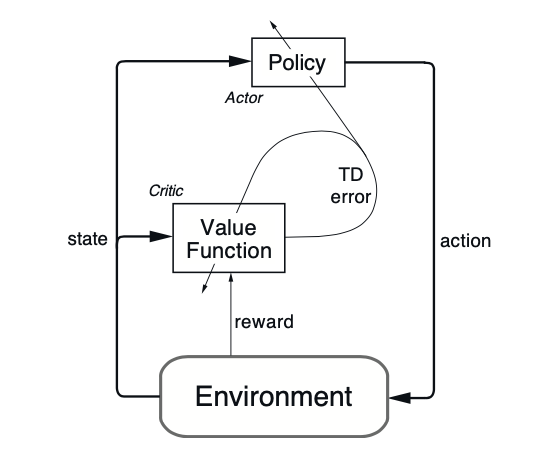
\includegraphics[height=5cm, width=0.4\linewidth]{actor-critic.png}
	\caption{Actor-critic system as depicted in \cite{SuttonBarto}}
	\label{fig:actor critic}
\end{figure}

This class of methods are naturally off-policy due to the use of the value-learner which are off-policy evaluators. Typically, each learner is represented by a deep neural network with policy-learner parameterized by $\theta$ and value-learner parameterized by $\phi$. \\

\textbf{DDPG:} At the basic level, DDPG combines Deep Q-learning with some policy-learner. The Deep Q-learning portion of DDPG is modified for a continuous action space and therefore have the Q-function be differentiable with respect to the action chosen by the policy-learner. The algorithm is as follows

\medskip

\begin{minipage}{0.95\linewidth}
\begin{algorithm}[H]
  \SetAlgoLined
  \caption{DDPG (Q Actor-Critic)}
  \textbf{Input:} Initial policy parameters $\theta_0$, Q-function parameters $\phi_0$ \\
  Set target parameters equal to initial parameters $\theta_{\text{target}} = \theta_0$, $\phi_{\text{target}} = \phi_0$ \\
  \For{$t = 1,2,...$}{
  	Observe states $s$ and selection action $a$ according to policy-learner \\
  	Execute $a$ and observe $s', r$ and store transition in replay buffer $\mathcal{D}$ \\
  	Sample minibatch of transitions from $\mathcal{D}$ \\
  	Compute targets
 	\begin{equation*}
 	y = r + \gamma Q_{\phi_{\text{target}}}(s',\pi_{\theta_{\text{target}}}(s'))
 	\end{equation*}
 	Update Q-function and policy by one step of gradient descent using targets $y$ \\
 	Update target networks with
 	\begin{align*}
 	\phi_{\text{target}} & = \rho\phi_{\text{target}} + (1 - \rho)\phi \\
 	\theta_{\text{target}} & = \rho\theta_{\text{target}} + (1 - \rho)\theta
 	\end{align*}
  }
  \KwResult{$\theta^*$ that parameterizes a mapping of states to actions, $\phi^*$ that parameterizes a mapping of state, action pairs to values}
  \label{algo:PPO}
\end{algorithm}
\end{minipage}

\medskip

Note this algorithm includes two tricks to help achieve stable convergence. First is maintaining a replay buffer of transitions $\mathcal{D}$ that ensure more stable updates to network parameters like how batching in SGD improves speed of convergence. Second, this algorithm introduces target networks that are separate from our training networks such that the targets no longer share the same parameters as our estimates. This prevents unstable minimization coming from feedback loops caused by parameter sharing. For further reading, see \cite{Silver2014} and \cite{Lillicrap2019}. \\

\textbf{A2C:} A2C is another actor-critic method that is a synchronous version of Asynchronous Advantage Actor Critic (A3C) released by DeepMind. The system is very similar to DDPG, however, we now have the value-learner approximating the advantage function rather than the Q-function. Approximating the advantage rather than the Q-value function increases stability by reducing the size of the rewards, leading to smaller, more stable gradients. The algorithm updates for the synchronous algorithm proceeds exactly like the DDPG algorithm above by replacing updates to the Q-function with updates to the advantage function. For further reading, see \cite{Mnih2016A2C}.

\section{Training Methods} \label{methods}

\subsection{Data}

It is well known that a model is only as good as the data it was trained on and this is especially the case in finance where different securities exhibit different price patterns and therefore require different trading strategies. Even similar products will have different behaviors depending on the specific seasonality or regulations of the underlying industry or products. 

To mitigate the effects of idiosyncratic events associated with single name stocks, we choose to train on ETFs that follow an industry or the market as a whole. Specifically, we chose the tickers SPY, XLE, XLF, XLI, XLK, XLV which track the S\&P500, energy, financial, industrials, technology, and healthcare sectors, respectively. This list is by no means exhaustive but offers a large coverage of sectors that each exhibit their own trends and thus would test the performance of our model in different environments.

For each ticker, the data is comprised of daily open, low, high, and close prices. The data was split into a training set and a validation set on the date 01/01/2015. That is the training set is all price data from when the ETF was created (1993 for SPY and 1998 for all others) to the end of 2014 and the validation set is all data from the start of 2015 through March 2021. Feature vectors were then created from the price data as follows:

\begin{itemize}
	\item Each price was adjusted for dividends
	\item Prices were lagged up to 5 days out and all prices were normalized as a percent change relative to the opening day of the first day (i.e. opening price of first day is 0)
	\item Exponential moving averages were calculated at each time step for window sizes of 5, 20, 50
\end{itemize}

These features were combined with current agent stock and cash holdings for a total of 28 features the agents used for their policy mappings. The same set of features (without stock and cash holdings) were used in estimating returns through GPR.

\subsection{Base Agents}

The base trading agents were trained using the \href{https://github.com/hill-a/stable-baselines}{stable baselines package} which provides high-quality implementations of various RL algorithms (\cite{stable-baselines}). Several algorithms were tested for performance including A2C, PPO, DDPG, and Deep Q-Learning. Of these, the A2C algorithm was chosen due to more consistent performance in achieving higher P\&L.

Agents were trained in a custom OpenAI \code{gym} environment that simulates daily trading of the underlying security. We restrict the action-space to be within trading 10 shares in either direction (buy or sell) for ease of exploration but this can be scaled up easily by either adding trade size multipliers or expanding the action-space directly. We assume the size of the trades are small in comparison to total daily trading volume and is therefore able to execute trades with negligible slippage.

Performance of the base agent can be seen in Figure \ref{fig:rl base}. We see the RL agent is able to achieve P\&L greater than the simple buy-and-hold strategy while learning to take long-only positions despite no restrictions on shorting. This indicates the agent has learned over time the stock price tends to go up and balances this long-term reward with the short-term losses it may incur.

\begin{figure}[H]
	\centering
	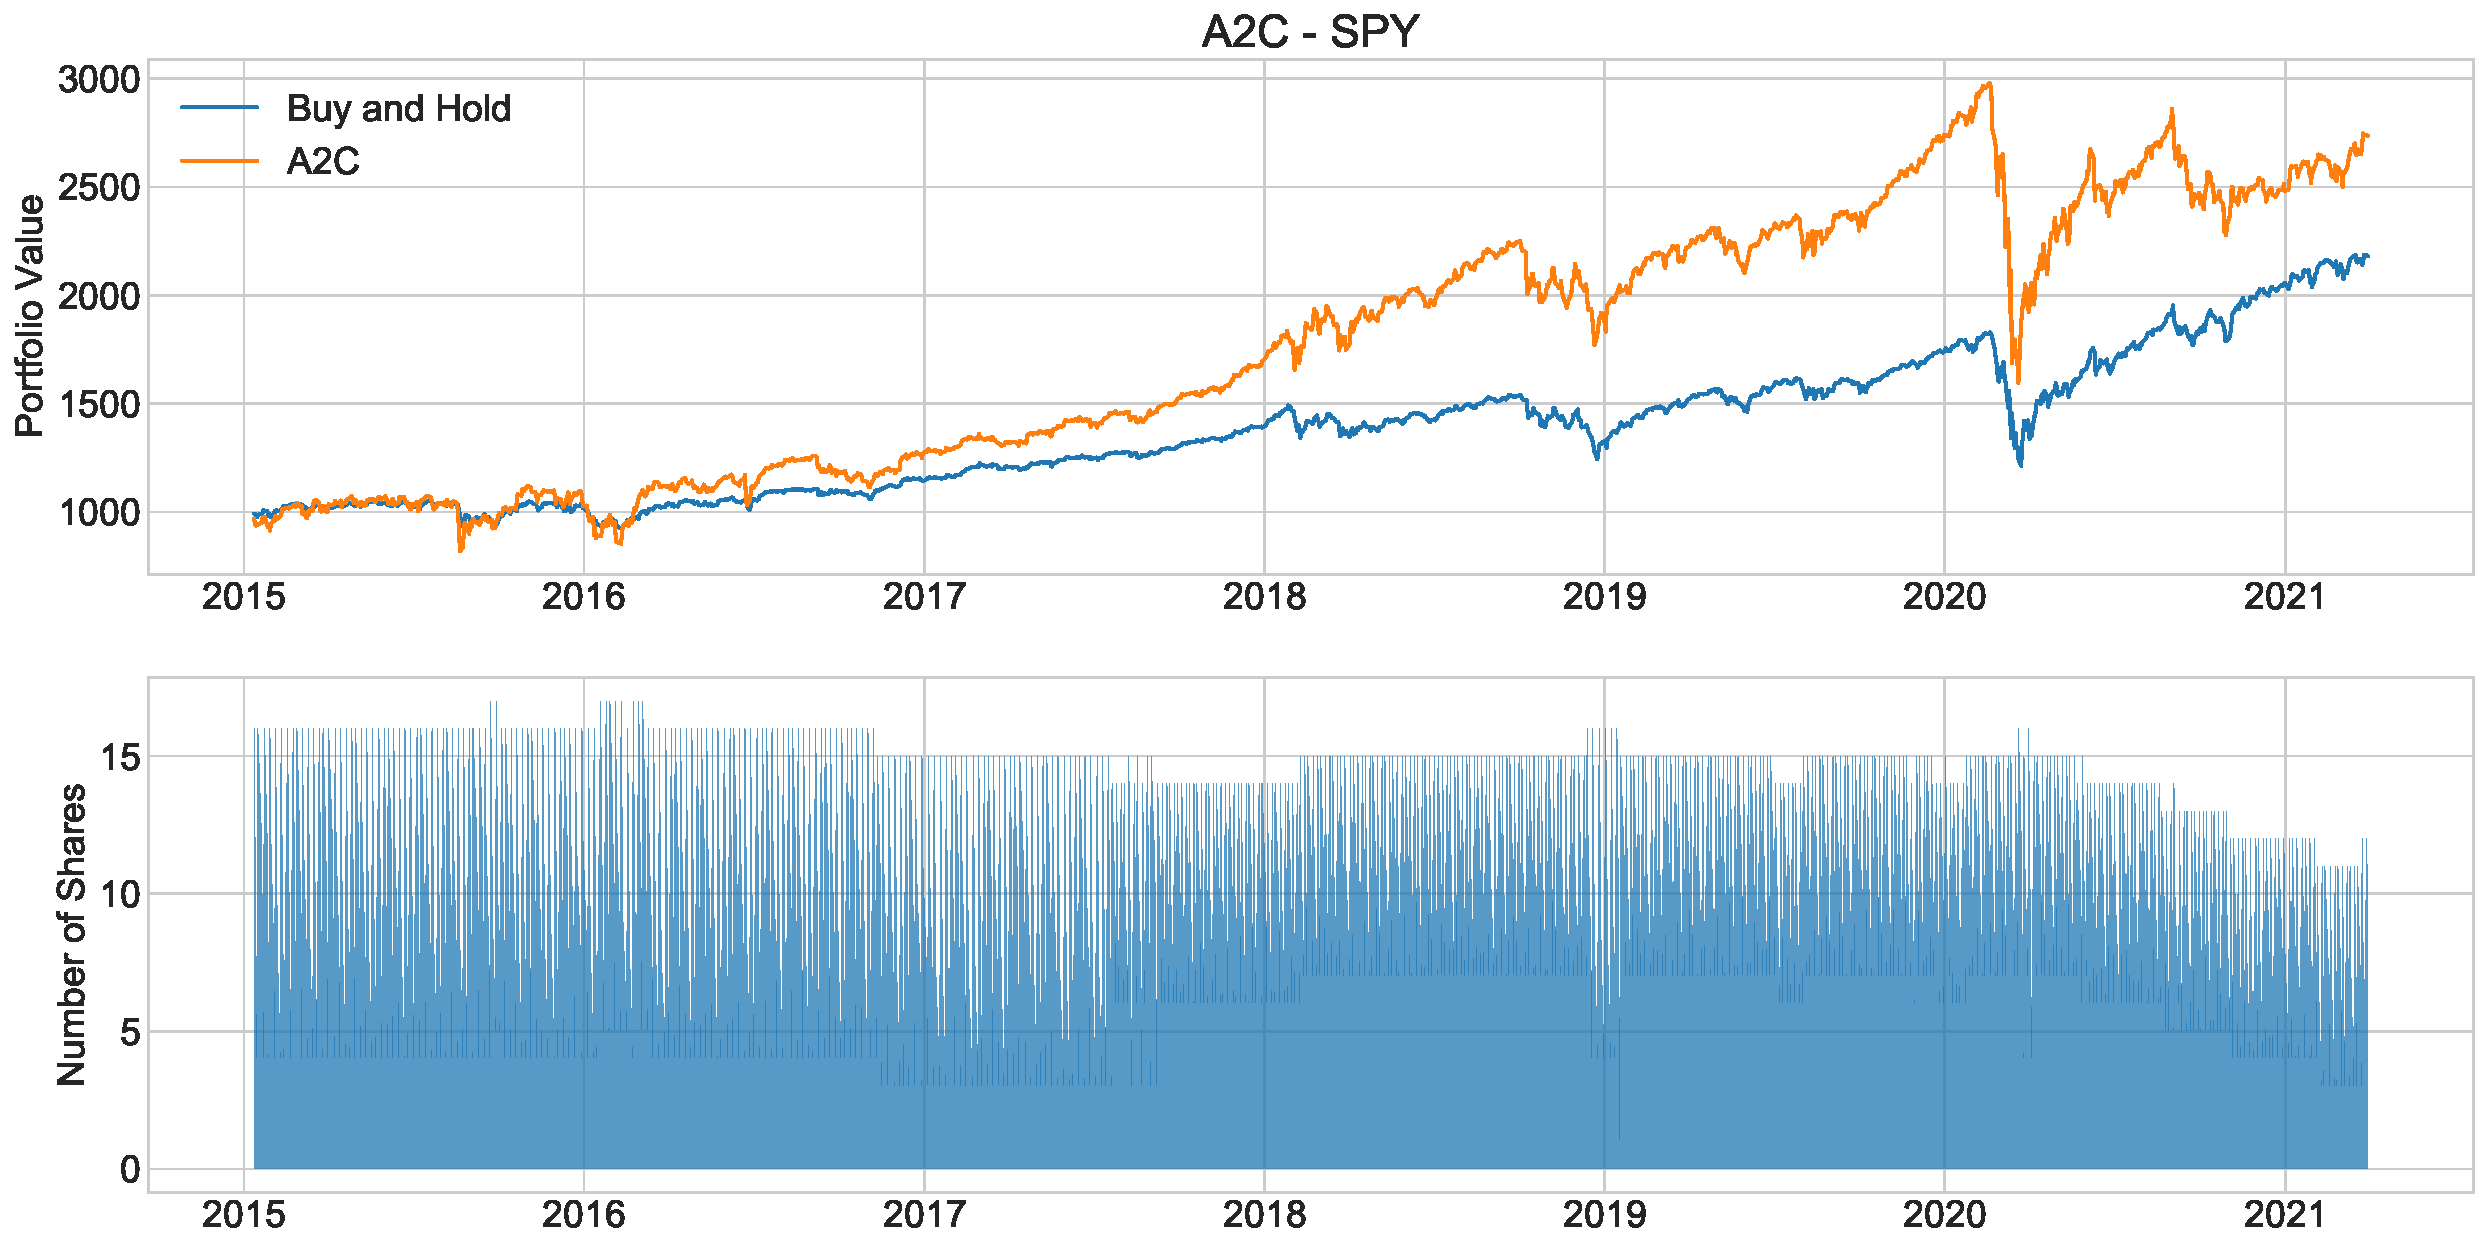
\includegraphics[width=\linewidth]{../src/figures/rl_base_no_restrictions.pdf}
	\caption{\textbf{Top image:} Performance of base RL agent compared to buy-and-hold strategy. \\ \textbf{Bottom image:} Number of shares held in agent's portfolio. Notice shares are strictly positive despite no restrictions on shorting.}
	\label{fig:rl base}
\end{figure}

\subsection{Risk Adjustment}

GPR is used to estimate the CVaR risk measure at every step and adjust trade size and direction to stay within a predetermined risk tolerance which was set to -0.05. An exact GP model with a scaled rbf kernel is used. The parameters of GPR are tuned in pretraining on an initial training set. At every step, the training examples used to train the GPR are updated. We use a lookback window of one month (20 trading days) for the training set. After the update, a small amount of training is done to tune the parameters to the new examples and a prediction of next step returns, a sample from the posterior, and confidence intervals are obtained.

If the magnitude of the mean prediction is greater than some pre-defined threshold (indicating relatively confident prediction), we adjust the RL agents action based on our predicted confidence intervals and predetermined risk tolerance as follows:

\begin{enumerate}
	\item Calculate CVaR per share for a long (short) position by approximating using set of samples from posterior below (above) the lower (upper) bound of the confidence interval
	\item Determine target number of shares in portfolio based on the per share CVaR
	\item Trade in direction of the target number of shares up to a maximum of 10 shares (to match the action restriction of the base RL agent)
\end{enumerate}

In this way, the GPR is essentially used to maintain a constant exposure by adjusting the size (and sometimes direction) of the base RL agent's actions. The results of these adjustments can be seen in Figure \ref{fig:rl with gp} where the agent position fluctuates less and even goes negative with sufficiently negative predicted returns. Note that these thresholds were tuned specifically for SPY and thus performance for SPY is illustrated. This may mean that performances are suboptimal for other instruments the algorithm was tested on.

\begin{figure}[H]
	\centering
	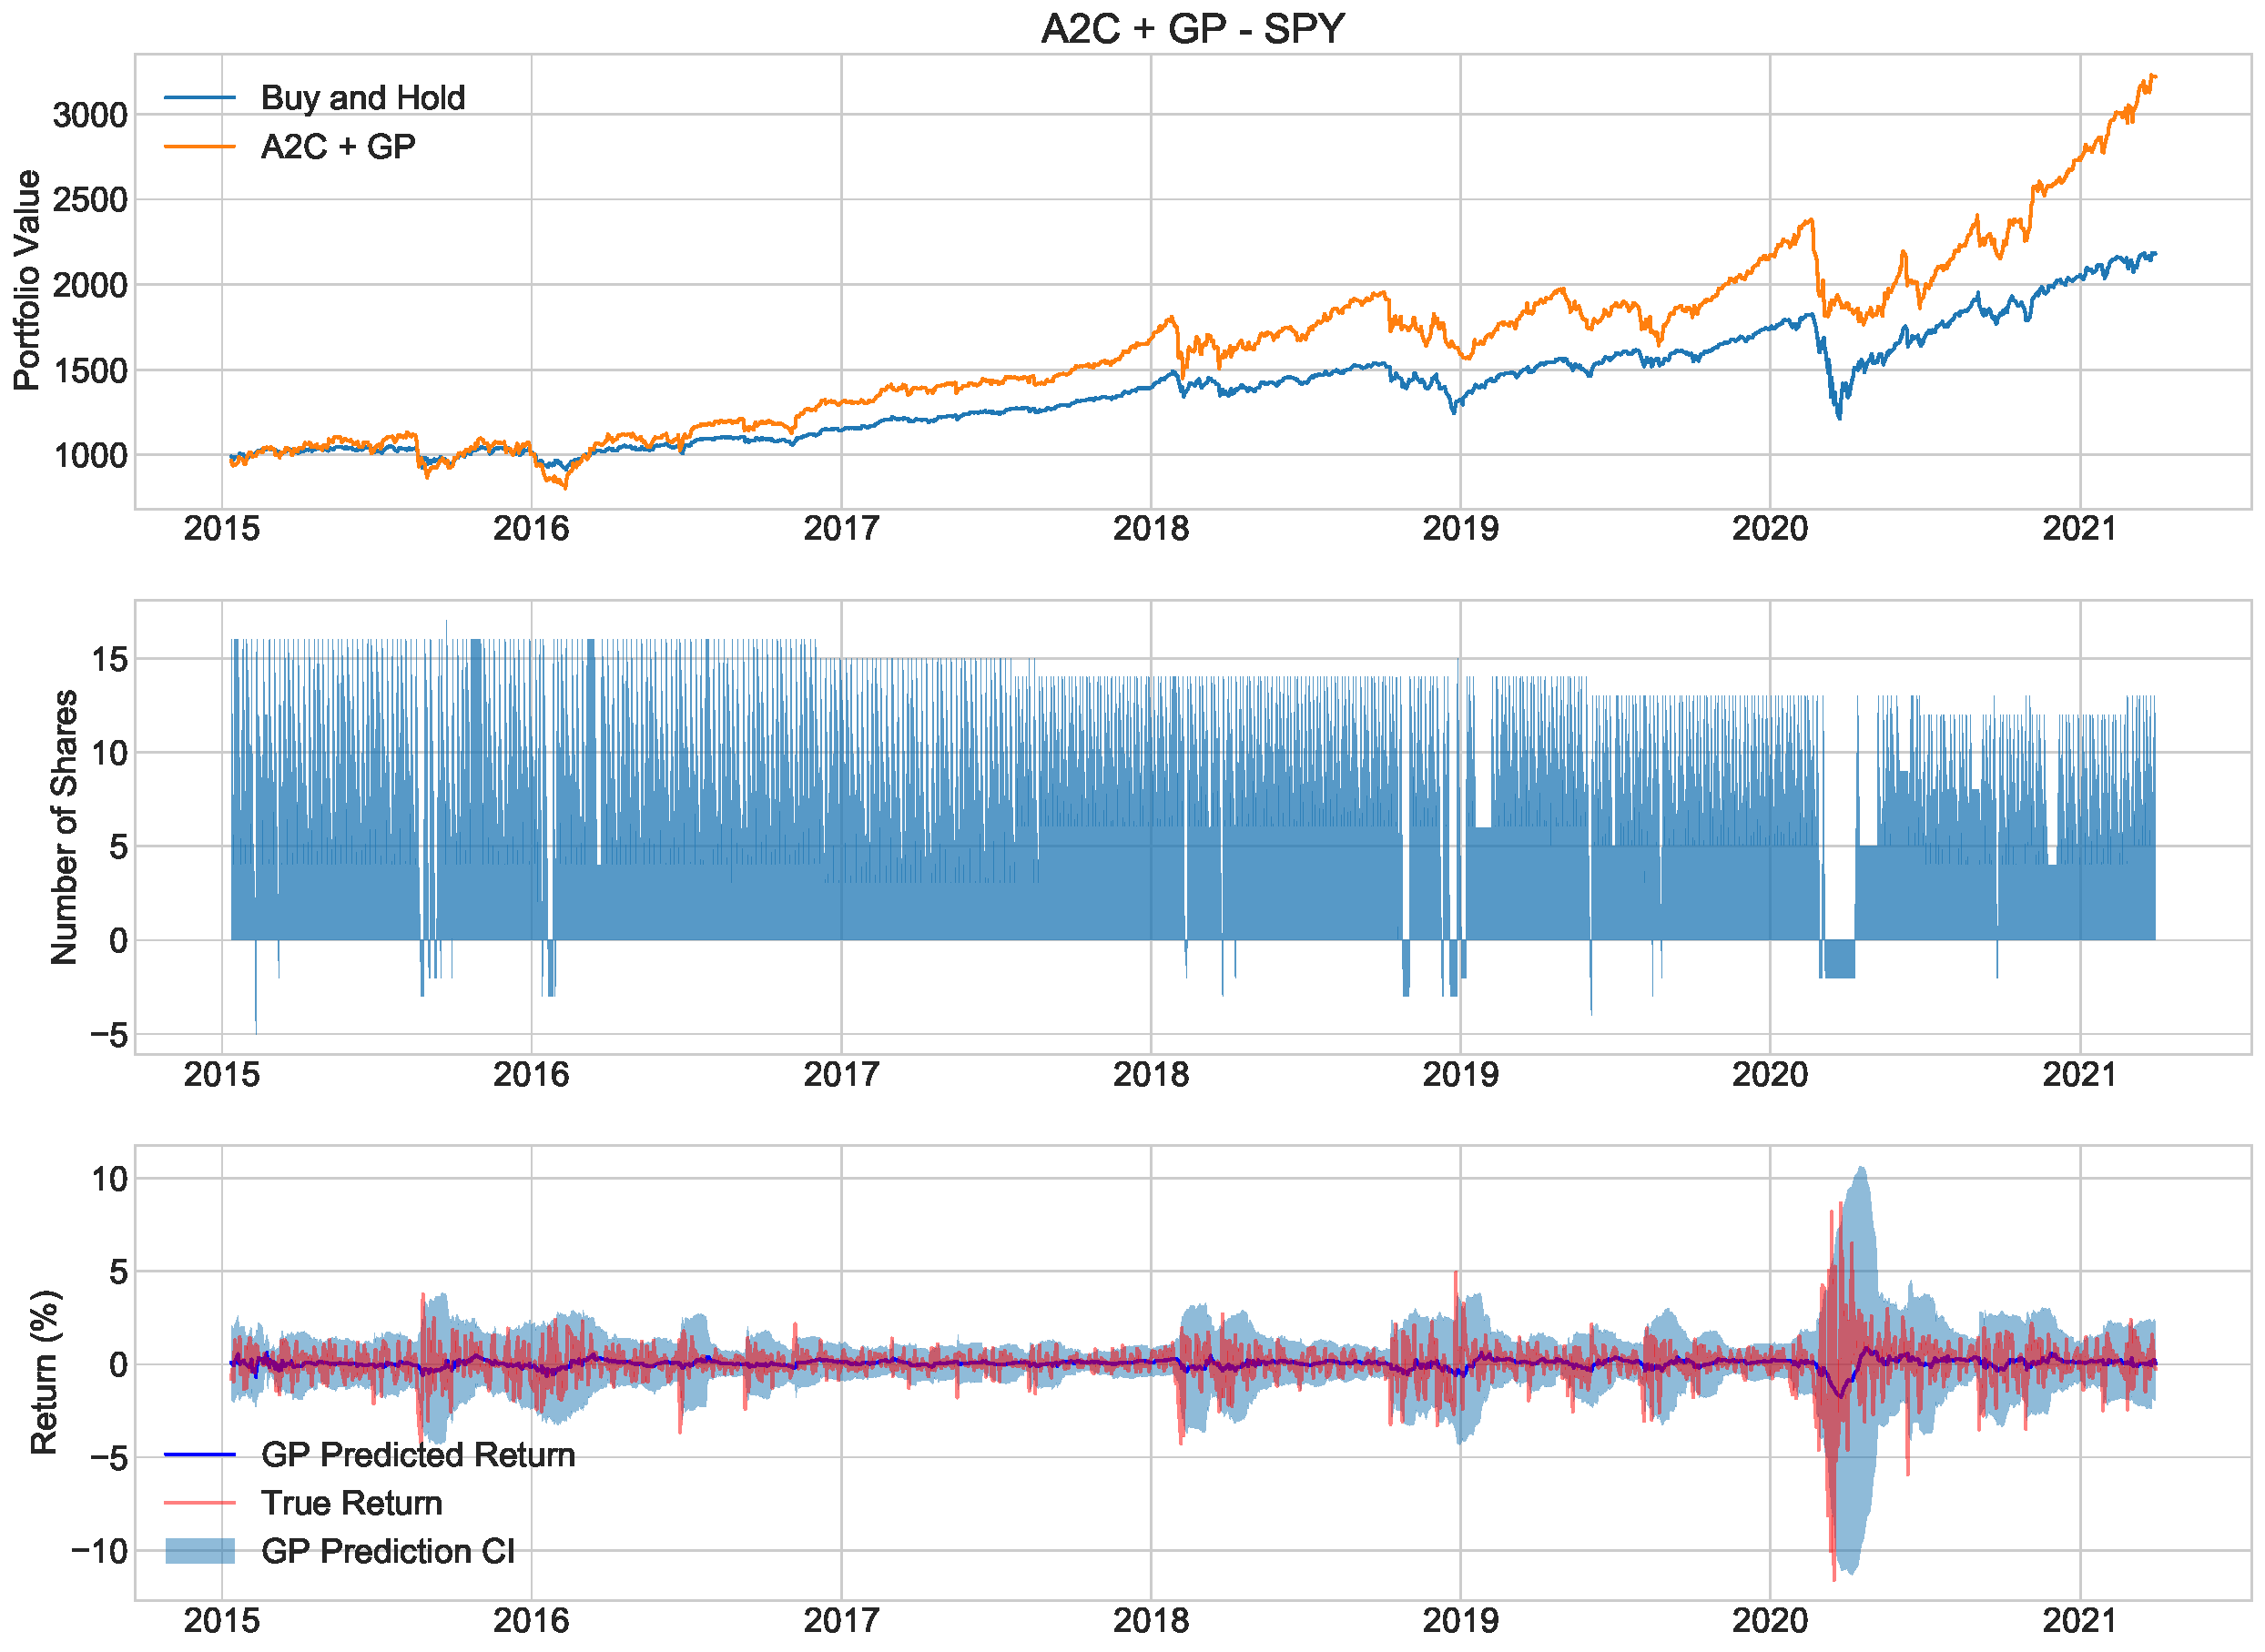
\includegraphics[width=\linewidth]{../src/figures/rl_with_gp_no_restrictions.pdf}
	\caption{\textbf{Top image:} Performance of RL agent with GPR adjustment compared to buy-and-hold strategy. \\ \textbf{Middle image:} Number of shares held in agent's portfolio. We see shares are now sometimes negative due to GPR returns prediction. \\ \textbf{Bottom image:} Predicted vs Observed returns and confidence intervals associated with the predicted value.}
	\label{fig:rl with gp}
\end{figure}

In Figure \ref{fig:rl with gp}, we see that the mean predictions of the returns follow the general direction of returns but are not very accurate which is expected given how noisy returns are. However, this is not seen as a major problem since we are less interested in the mean estimates and are rather focused on the confidence intervals of the posterior. We see the confidence intervals approximate the observed volatility well which indicates the use of these confidence intervals for risk measure estimation is valid.

\subsection{Risk Metrics}

We use a few metrics commonly seen in industry to assess the performance of our algorithms. P\&L as measured by annualized returns is the first point of comparison since the root of the problem is whether these algorithms make money trading. Also in line with intuition, the higher this annualized return, the better. However, this does not account for the risk being taken to achieve the P\&L. Typically, higher returns come from riskier investments. Therefore, it is important to measure the efficiency of the positions with respect to the risk being taken. For this, the Sharpe ratio is commonly used. For an investment $X$, given some risk-free rate (assumed 0 for our purposes) the Sharpe ratio is given by

\begin{equation}
SR(X) = \frac{\E[R_X - R_f]}{\sigma_X}
\label{eq:sharpe}
\end{equation}

Where $R_X$ is the return of the investment, $R_f$ is the risk-free rate, and $\sigma_X$ is the volatility of the investment. Intuitively, the Sharpe ratio measures the additional returns gained from taking on an additional unit of risk as measured by its volatility. Higher Sharpe ratios suggests greater efficiency of risk being taken.

An additional point of concern in trading is sustained loss over a period of time or drawdown. Drawdown measures decline from a previous peak of some portfolio. If $P$ is our portfolio value and is indexed by time $t$, then the drawdown $D$ at time $T$ is given by

\begin{equation}
D(P) = \max_{t\in(0,T)}P(t) - P(T)
\label{eq:drawdown}
\end{equation}

This is an especially relevant concern for fund managers who risk investor withdrawals given large enough losses. Therefore, an algorithm that achieves high P\&L in the long run but suffers large drawdowns may not have the chance to achieve the later successes due to investor withdrawals. Thus, smaller drawdowns indicate better strategy performance.

\section{Results} \label{results}

As previously stated, the parameters such as the weights of the RL agent and those in the kernel function of the GPR are trained separately for each ticker we test on. The threshold for GPR intervention was only tuned for SPY and then used for all tickers. The main focus of the study was on SPY as it is the main market being tracked and experiences less idiosyncratic events that could affect specific sectors. The GP-augmented strategy is compared against the raw RL agent and the passive buy-and-hold strategy. The results are summarized in Table \ref{tab:results summary} where the best performing strategy is bolded for each ticker for each metric.

We see that for SPY, our GP-augmented strategy had the best performance by every metric achieving the highest annualized returns, highest Sharpe ratio, and lowest max drawdown. This indicates that the algorithm is able to more efficiently take risks and produces more stable trading compared to the simple buy-and-hold strategy.

The results for other tickers are more mixed, as the GP-augmented strategy far outperforms the other strategies on XLE but underperforms on XLI. And while achieving highest returns and Sharpe ratio for three of the five sector ETFs and was close on a fourth, it consistently failed to produce smaller max drawdowns compared to the simple buy-and-hold strategy. However, it is important to note that the GP-augmented strategy did achieve lower max drawdowns than the raw RL agent and thus combined with the higher Sharpe ratio indicates an improvement in terms of riskiness of positions.

\begin{table*}[t]
	\centering
	\begin{tabular}{c|c|c|c c c c c c}
	\hline
	& Strategy & SPY & XLE & XLF & XLI & XLK & XLV \\
	\hline
	Annualized Returns & Buy and Hold & 13.37 & -2.83 & 11.64 & 11.98 & 22.24 & 10.33 \\
	(\%) & A2C & 17.60 & 2.55 & \textbf{17.71} & \textbf{17.36} & 29.25 & 14.94 \\
	& A2C + GP & \textbf{20.73} & \textbf{16.99} & 16.85 & 13.43 & \textbf{30.90} & \textbf{15.99} \\
	\hline
	Sharpe Ratio & Buy and Hold & 0.6773 & -0.1104 & \textbf{0.4374} & \textbf{0.5147} & 0.8694 & 0.5534 \\
	(Annualized) & A2C & 0.5868 & 0.0045 & 0.3805 & 0.4417 & 0.7101 & 0.4367 \\
	& A2C + GP & \textbf{0.8624} & \textbf{0.3537} & 0.4352 & 0.3830 & \textbf{0.9953} & \textbf{0.5750} \\
	\hline
	% Total Returns & Buy and Hold & 117.96 & (16.31) & 98.11 & 101.94 & 248.08 & 84.16 \\
	% (\%) & A2C & 173.65 & 16.90 & \textbf{175.30} & \textbf{170.19} & 392.13 & 137.43 \\
	% & A2C + GP & \textbf{222.23} & \textbf{165.05} & 163.02 & 118.67 & \textbf{432.39} & \textbf{151.27} \\
	% \hline
	Max Drawdown & Buy and Hold & (33.71) & (62.99) & \textbf{(42.86)} & \textbf{(42.33)} & \textbf{(31.15)} & \textbf{(28.40)} \\
	(\%) & A2C & (46.40) & (115.96) & (59.71) & (59.09) & (39.93) & (48.89) \\
	& A2C + GP & \textbf{(29.18)} & \textbf{(60.61)} & (55.16) & (46.48) & (34.61) & (36.98) \\
	\hline
	\end{tabular}
	\caption{Back-testing metrics for trading period 1/1/2015 - 3/30/2021}
	\label{tab:results summary}
\end{table*}

Figures \ref{fig:spy perf comp} and \ref{fig:spy dd comp} shows the performance over time of the different strategies trading on SPY. We see that in terms of portfolio returns, the relative performance of the strategies changes with the time period. For example, the raw RL agent and the GP-augmented strategies both perform in line with the buy-and-hold strategy before outperforming it in the period of 2016 to 2018. Within this period, the two active strategies have roughly the same returns while the GP-augmented has lower drawdowns. However, the raw RL agent outperforms the GP-augmented in the period of 2018 to 2020. Finally, from 2020 on, the GP-augmented strategy outperforms the other two.

These discrepancies make sense given that often times markets experience regime shifts in which the dynamics of the market change and therefore so would the optimal trading strategy. In this experiment, the RL agents are deterministic and make no updates to their parameters at each step. The GP is able to make small adjustments as it re-trains its parameters partially at each step but the preset thresholds do not change. Therefore, the same algorithm would be expected to perform differently under different conditions. 

Looking specifically at the regimes of these different periods, we note that the period of 2015 to 2016 was a relatively quiet year focused around central bank policy and global growth. Why the active strategies weren't able to outperform the buy-and-hold strategy remains a mystery and would require further examination.

The period of 2016 to 2018 offered low volatility and general optimism from tax cuts to increasingly positive economic data. In such a case, it makes sense that the two active strategies outperform the passive strategy and perform in line with each other since the GP-augmented strategy has relatively little reason to intervene in periods of lowered risk.

The period of 2018 to 2020 was exhibited high volatility and general concerns of an upcoming recession. In this context, it makes sense for the more risk-aware agent (GP-augmented) to pare down positions and therefore experience lower returns than the unregulated raw RL agent. The larger drawdowns seem to be due to poor estimation of returns given the higher volatility that may be resolved by increasing the predetermined threshold.

Finally, from 2020 onwards we see increased volatility dominated by the recession caused by the COVID-19 pandemic. In this situation, the GP-augmented agent was able to mitigate losses experienced by the other strategies at the onset of the recession which helped it recover more quickly as the markets recovered. Further, it was better able to correctly predict market returns which helped it appropriately size up or down its positions. Why it was able to predict the returns in this period as opposed to the 2018 to 2020 period is unknown and would also require further examination.

Similar comparison figures are produced for each of the other tickers (\ref{fig:xle}, \ref{fig:xlk}, \ref{fig:xlv}, \ref{fig:xlf}, \ref{fig:xli}) as well as a plot of the volatility of SPY (\ref{fig:spy vol}) can be found in the appendix. While performance of our GP-augmented strategy varied by ticker, in almost all cases, the GP-augmented strategy was able to mitigate the largest drop in portfolio value (namely the March 2020 hit).

\begin{figure*}[t]
	\centering
	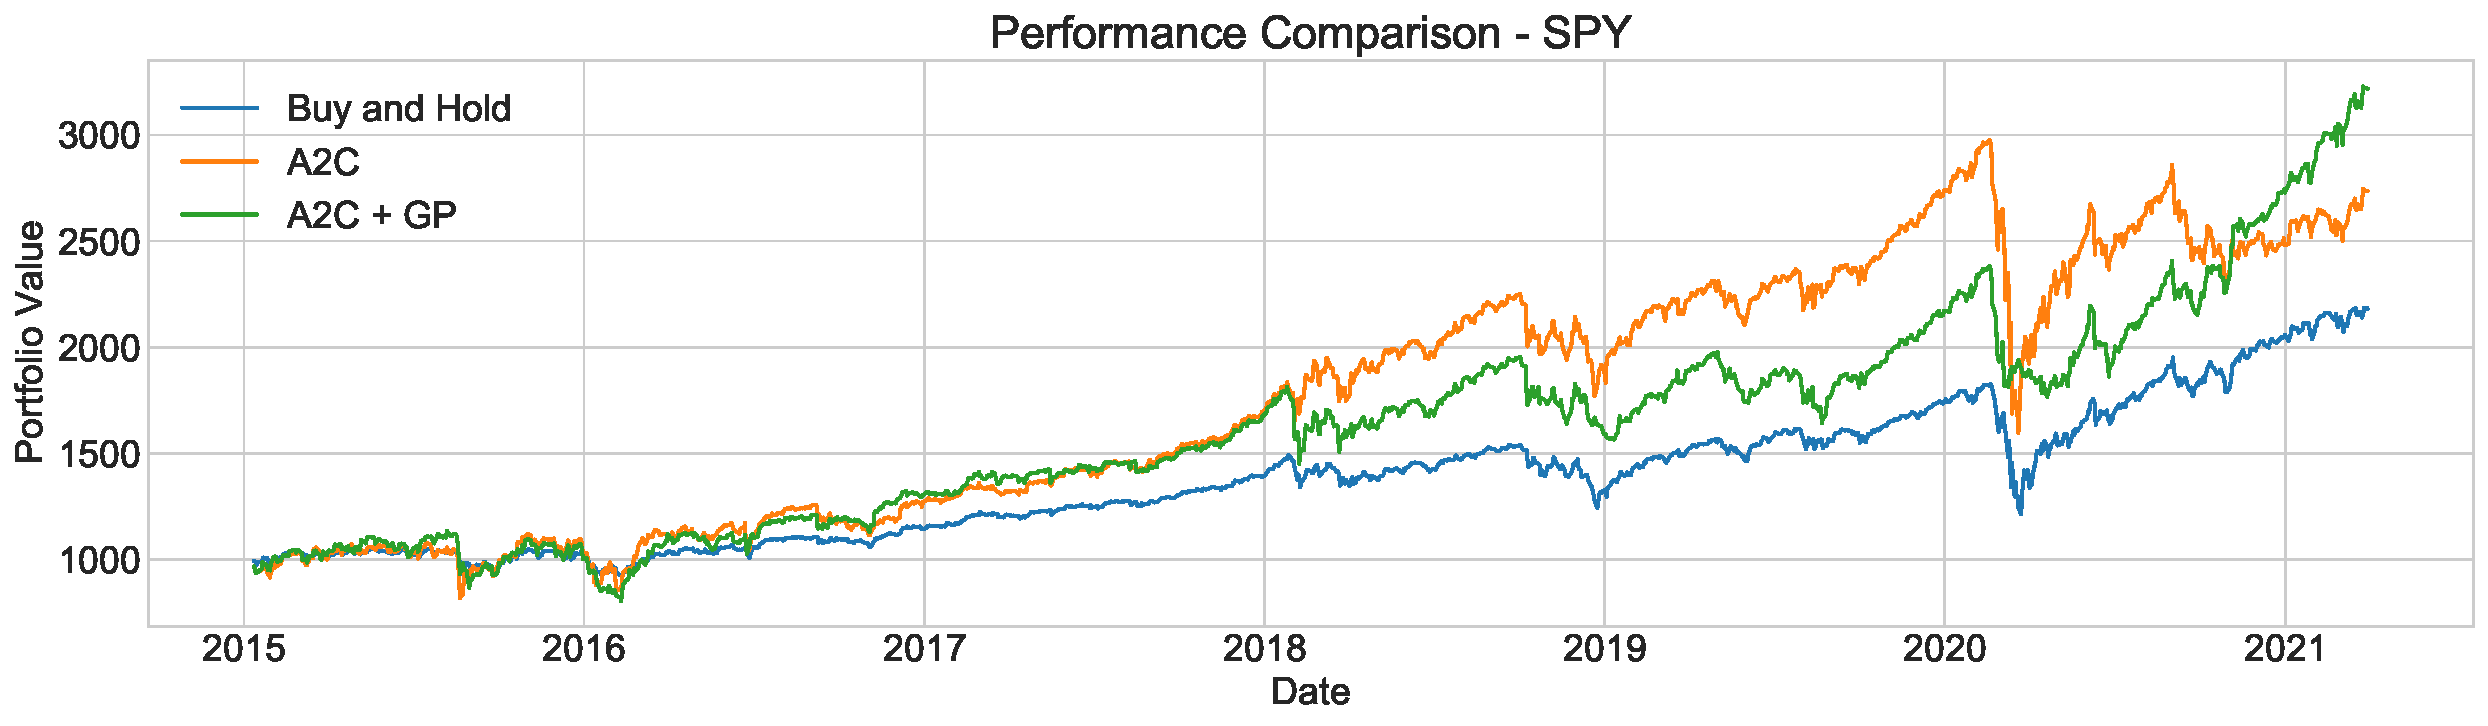
\includegraphics[width=\linewidth]{../src/figures/rl_gp_comparison_no_restrictions.pdf}
	\caption{This figure shows the portfolio values over time of an initial 1000 investment for the three strategies}
	\label{fig:spy perf comp}
\end{figure*}

\begin{figure*}[t]
	\centering
	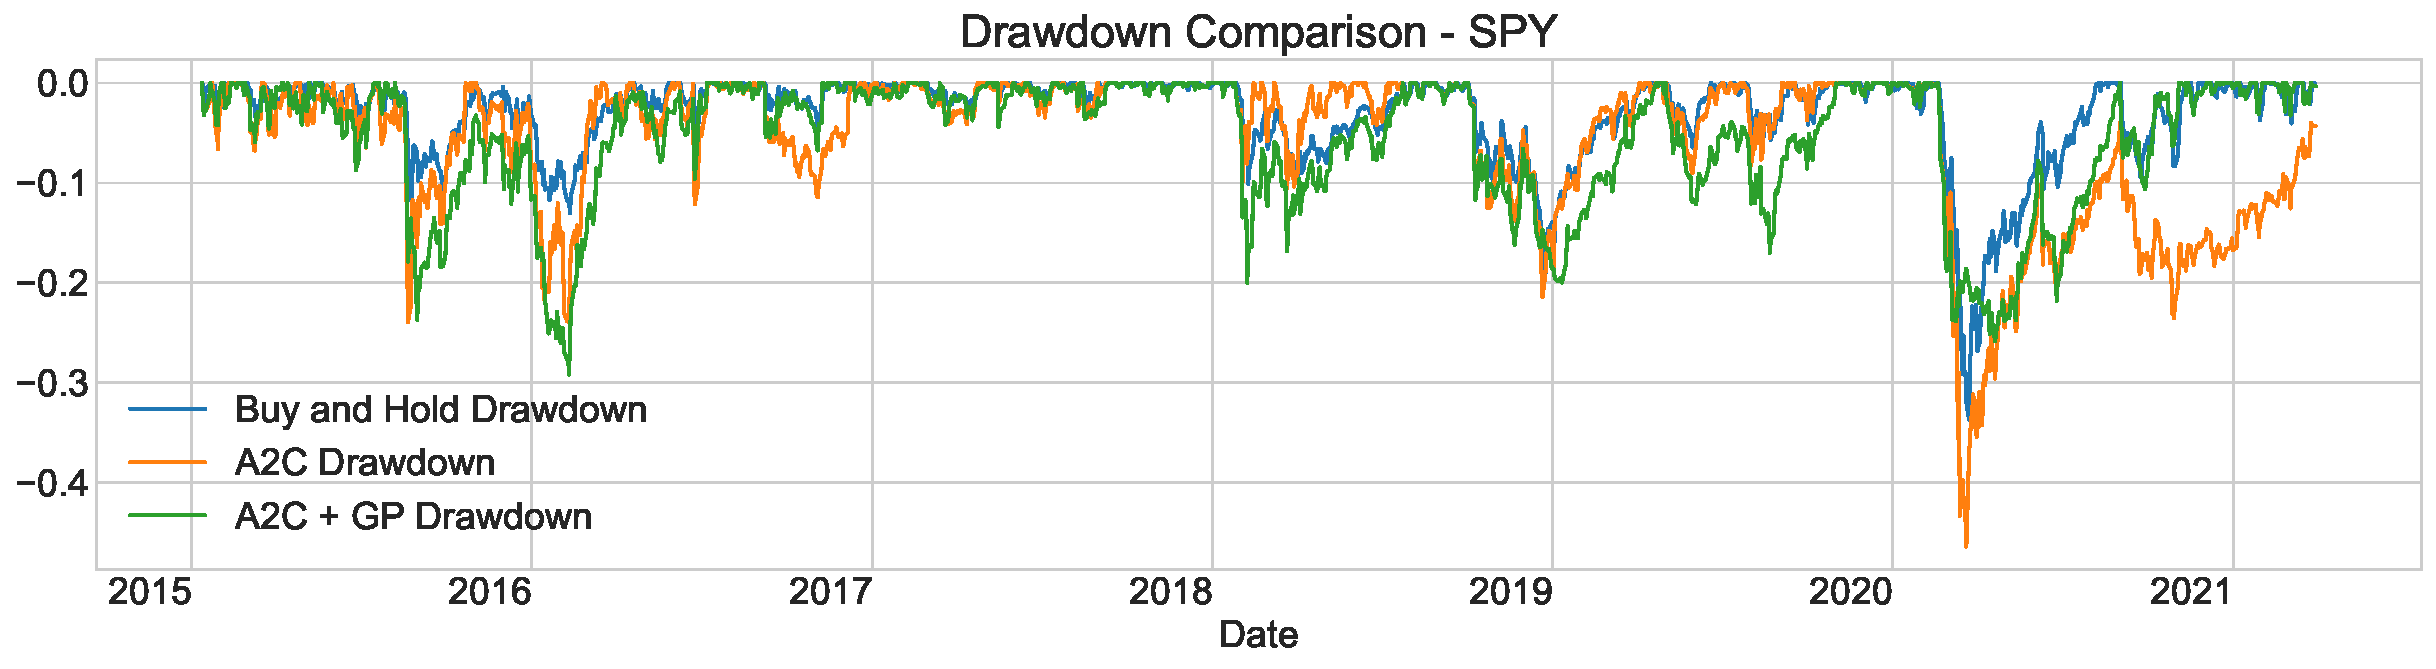
\includegraphics[width=\linewidth]{../src/figures/spy_drawdowns_comparison.pdf}
	\caption{This figure shows the comparison of drawdowns for each of the three strategies}
	\label{fig:spy dd comp}
\end{figure*}

\section{Conclusion} \label{conclusion}

Trading as an optimal control problem is a challenging one with clear benefits for even partial solutions. Casting it as a reinforcement learning problem allows for the application of state-of-the-art algorithms to discover optimal strategies through direct interactions within a simulated market environment. We manage the RL algorithms' tendencies to choose high reward over lower risk using a GPR for risk measure estimation and maintaining relatively constant risk exposures.

The results show that the GP-augmented strategy with properly tuned parameters is able to provide better performance as measured by annualized returns, Sharpe ratio, and max drawdowns over our back-test period. Without finely tuned threshold parameters, the GP-augmented strategy was still able to mitigate max drawdowns and often achieves higher Sharpe ratios. 

We recognize that the results are affected by the period over which we test. The GP-augmented strategy performs much better or worse depending on industry and market conditions subject to regime shifts. Based on this observation, a worthwhile extension would be to incorporate a simple regime change classifier that then switches between which strategy to follow.

This experiment shows the potential for this approach to improve the a pure RL trading strategy but further work can be done in extending both the features and the models used in this experiment. First, the feature space used is relatively basic and only includes some lagged price variables and some technical indicators. However, many informative technical indicators exist and experiments can be carried out to find the most informative subset of such features. In addition, the GP used in the estimation was an exact GP with a relatively simple kernel. Using approximate GP could provide more conservative risk measures and prevent some of the largerd drawdowns the GP-augmented strategy experienced. Choosing a more complex kernel could add to the accuracy of the returns and confidence interval predictions. Both of these improvements could provide avenues for improving the trading strategy.

% Create bibliography
\newpage
\bibliography{report}

\newpage
\section{Appendix}

\begin{figure*}[h]
	\centering
	\begin{subfigure}{\linewidth}
		\centering
		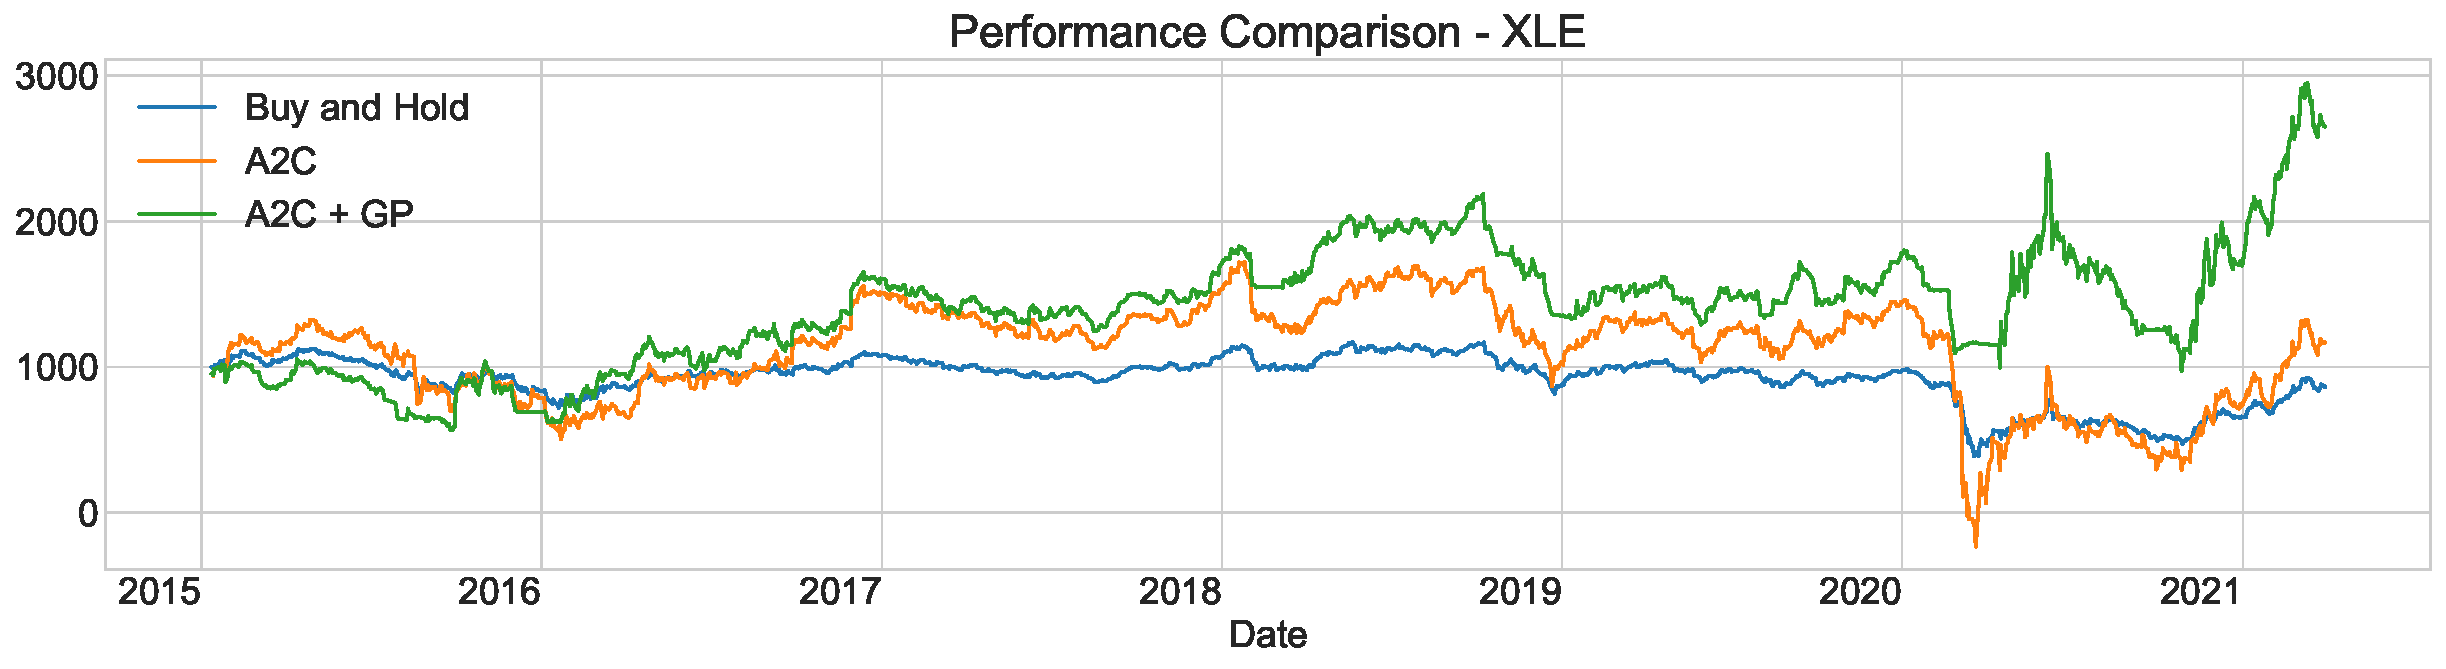
\includegraphics[width=\linewidth]{../src/figures/xle_performance_comparison.pdf}
	\end{subfigure}
	\begin{subfigure}{\linewidth}
		\centering
		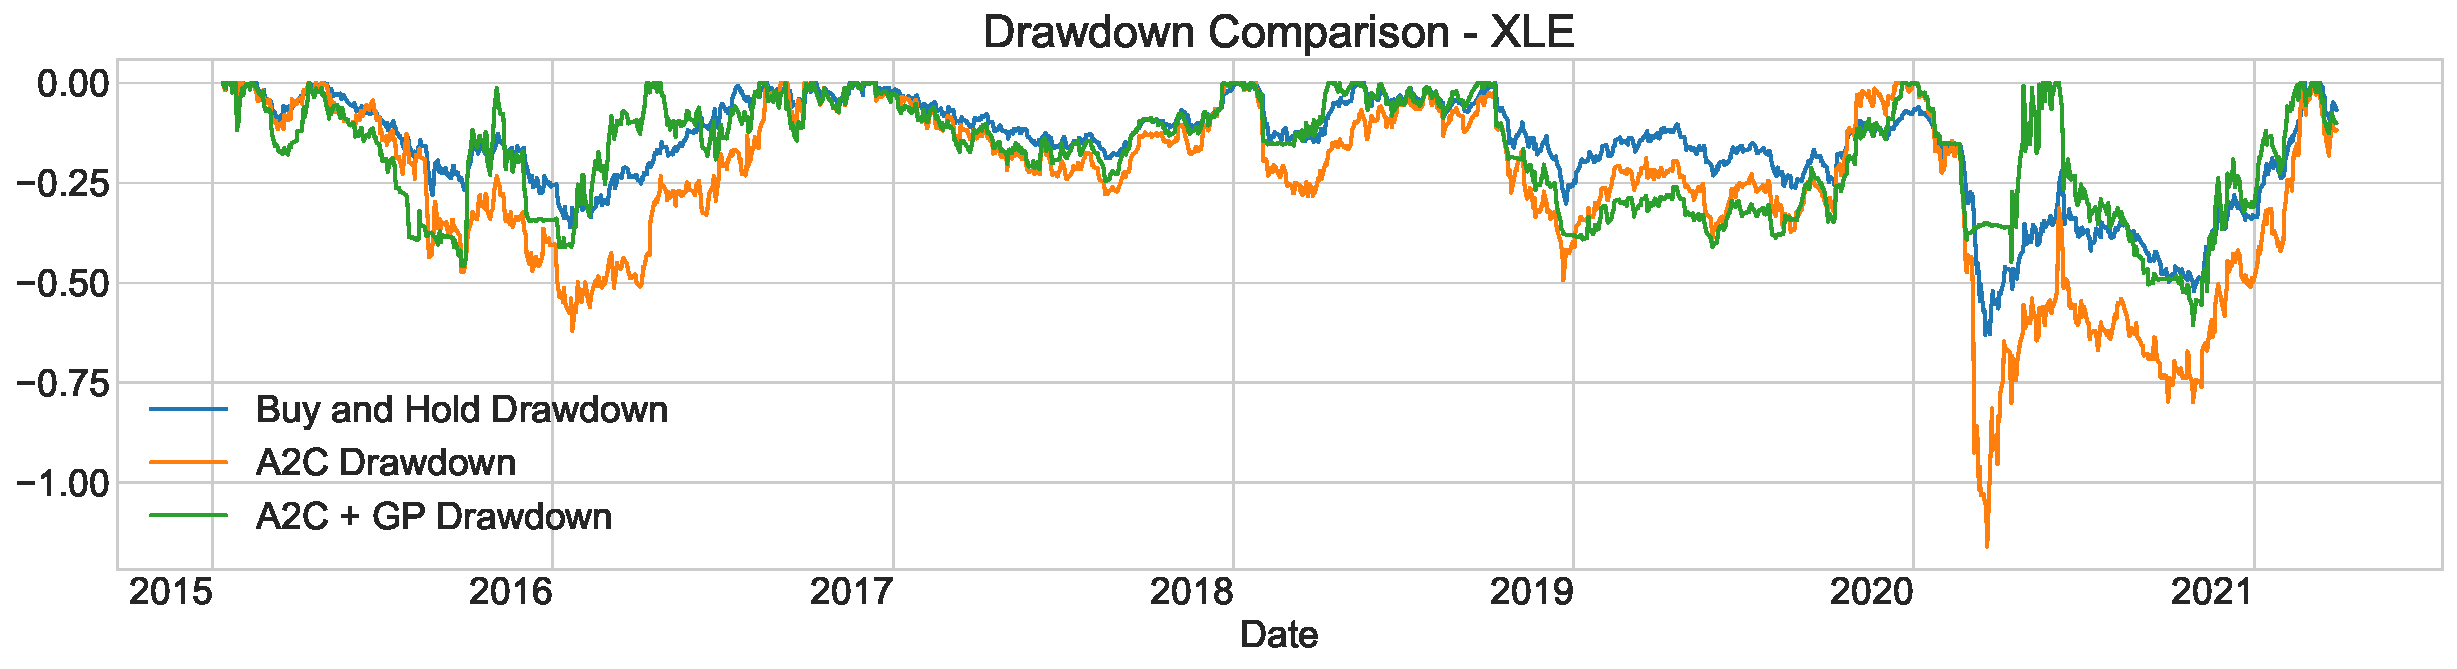
\includegraphics[width=\linewidth]{../src/figures/xle_drawdowns_comparison.pdf}
	\end{subfigure}
	\caption{}
	\label{fig:xle}
\end{figure*}

\begin{figure*}[h]
	\centering
	\begin{subfigure}{\linewidth}
		\centering
		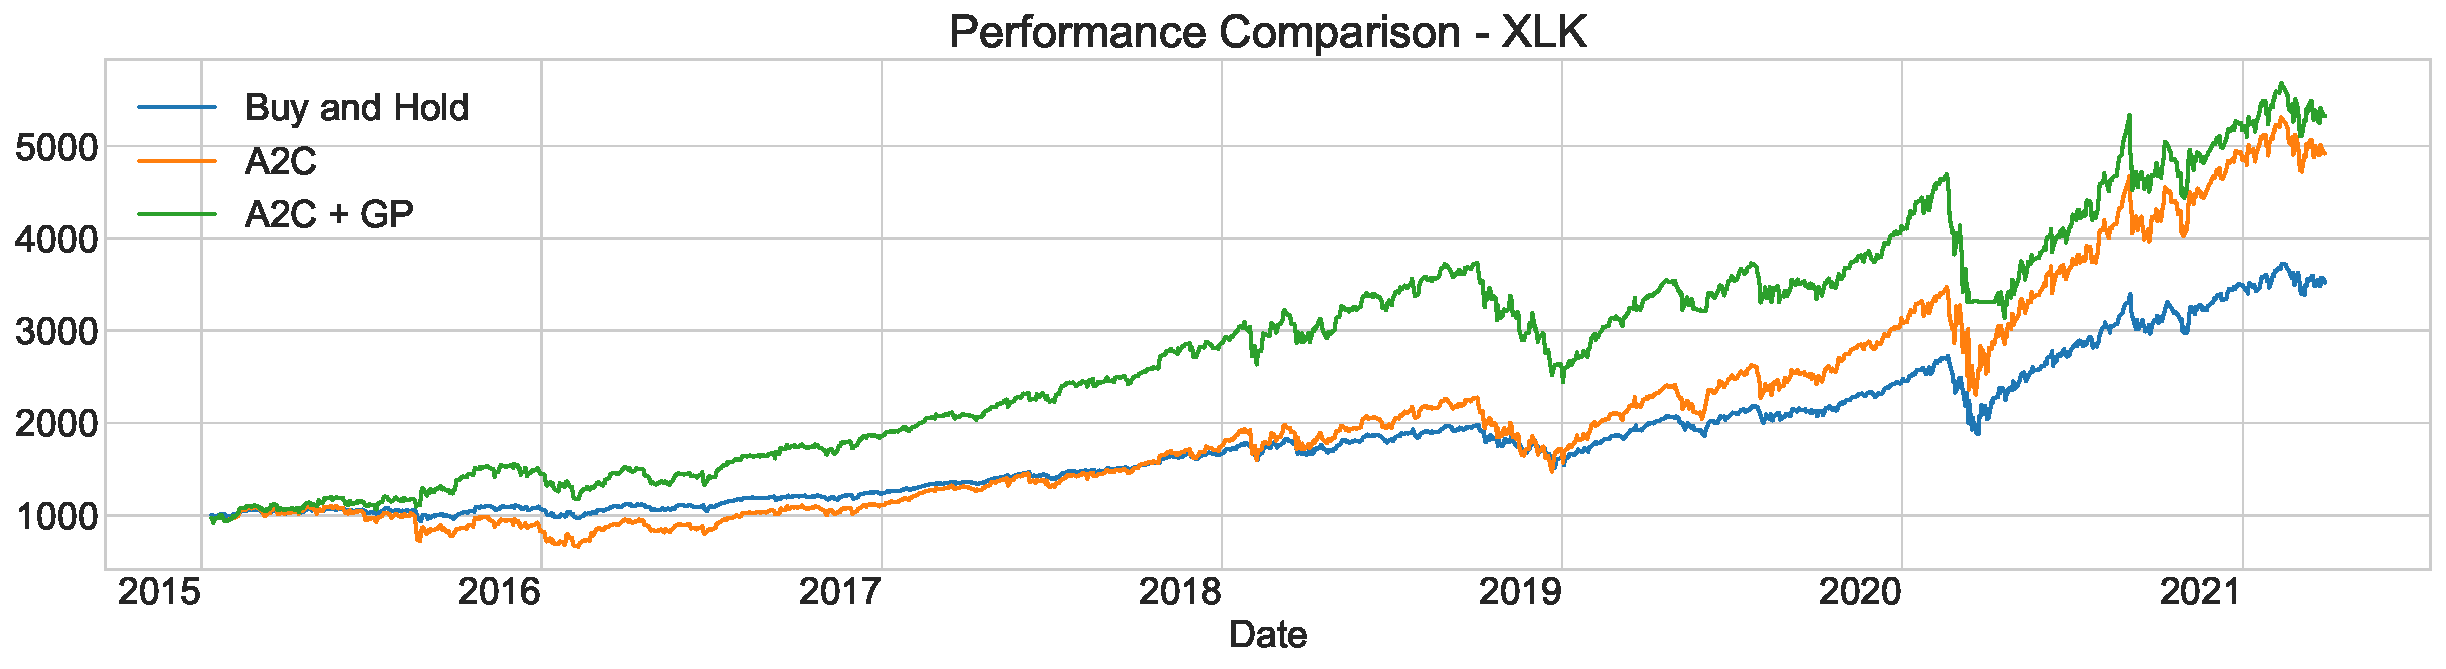
\includegraphics[width=\linewidth]{../src/figures/xlk_performance_comparison.pdf}
	\end{subfigure}
	\begin{subfigure}{\linewidth}
		\centering
		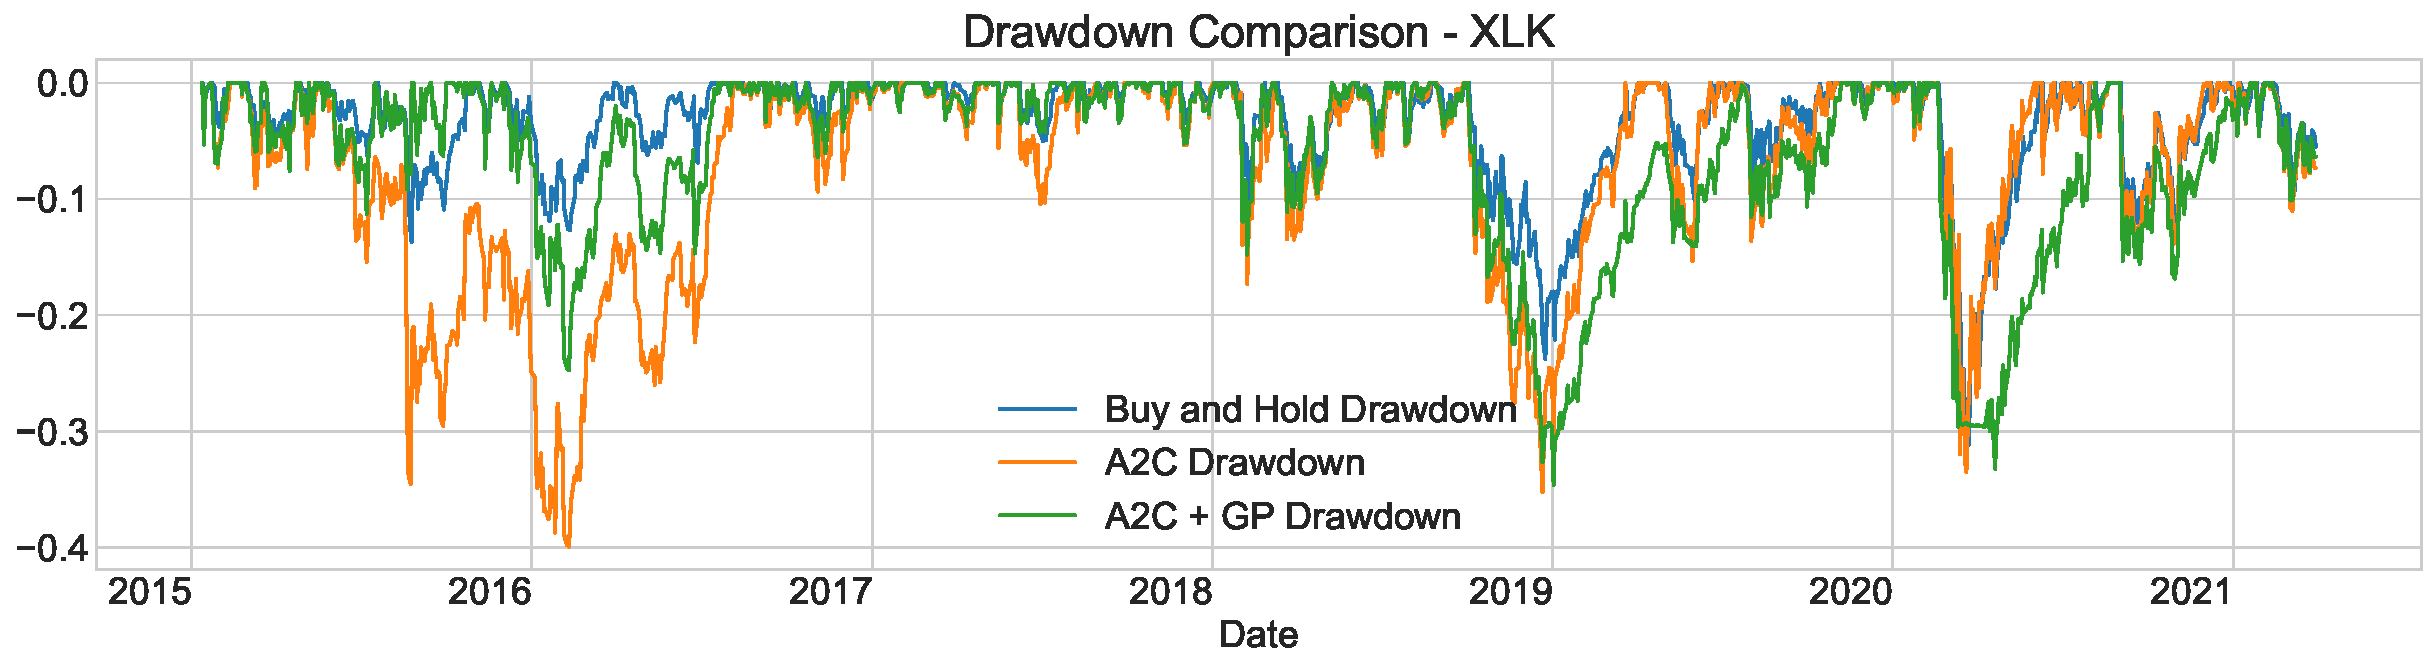
\includegraphics[width=\linewidth]{../src/figures/xlk_drawdowns_comparison.pdf}
	\end{subfigure}
	\caption{}
	\label{fig:xlk}
\end{figure*}

\begin{figure*}[h]
	\centering
	\begin{subfigure}{\linewidth}
		\centering
		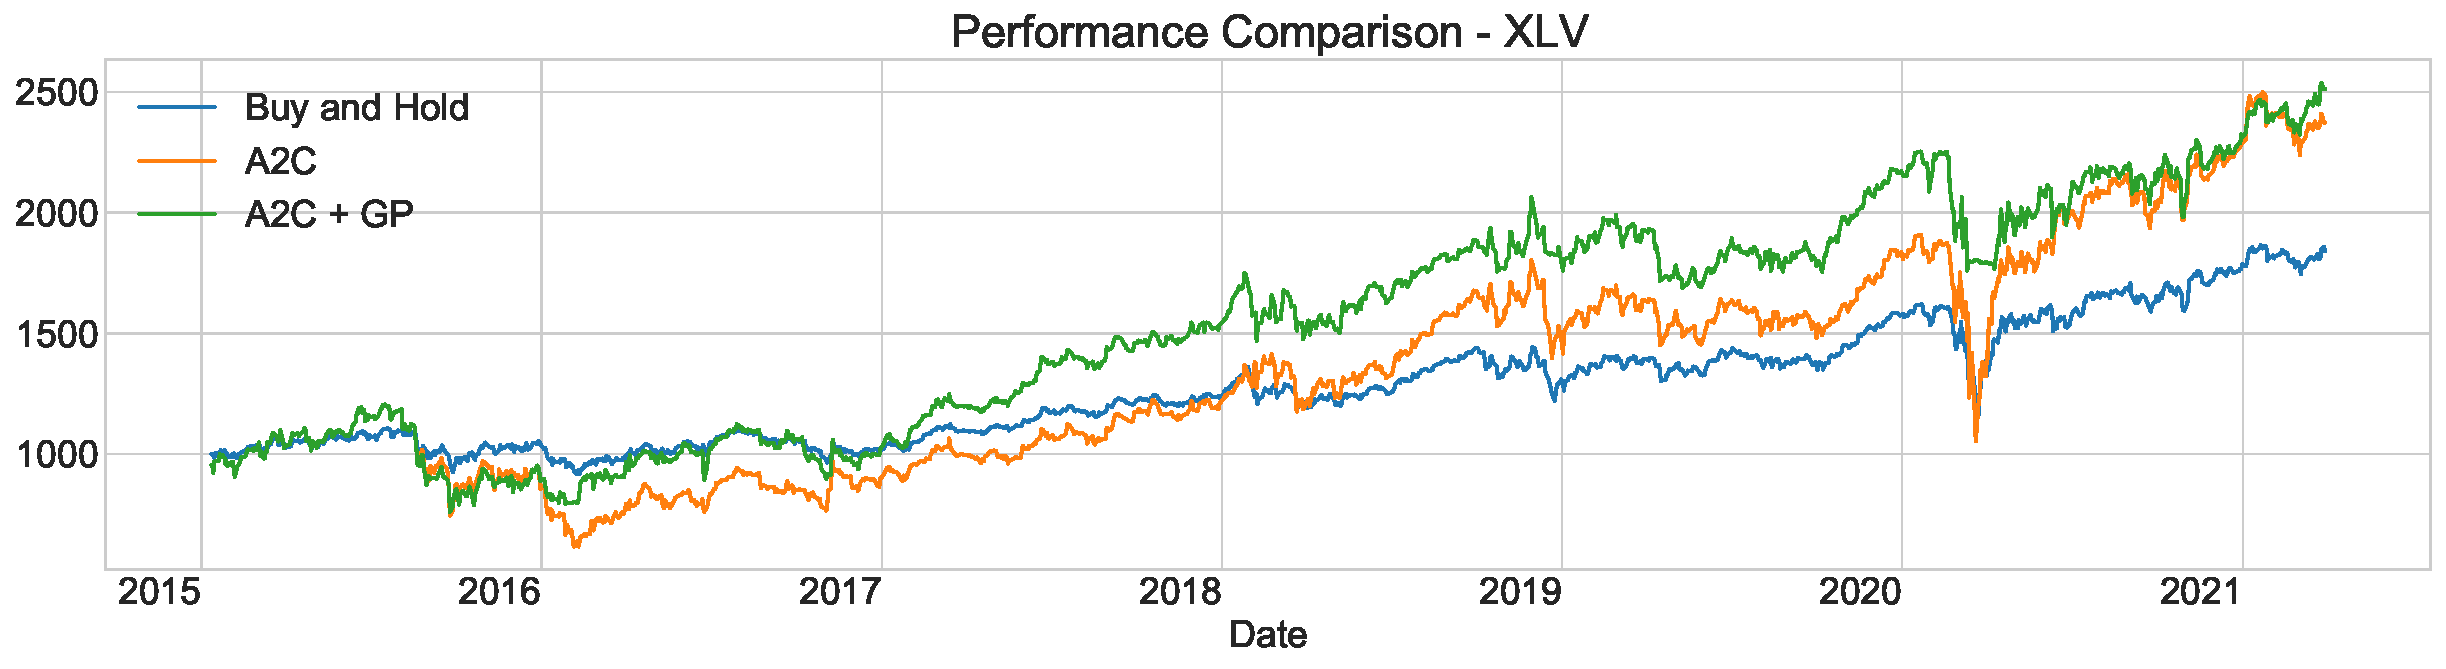
\includegraphics[width=\linewidth]{../src/figures/xlv_performance_comparison.pdf}
	\end{subfigure}
	\begin{subfigure}{\linewidth}
		\centering
		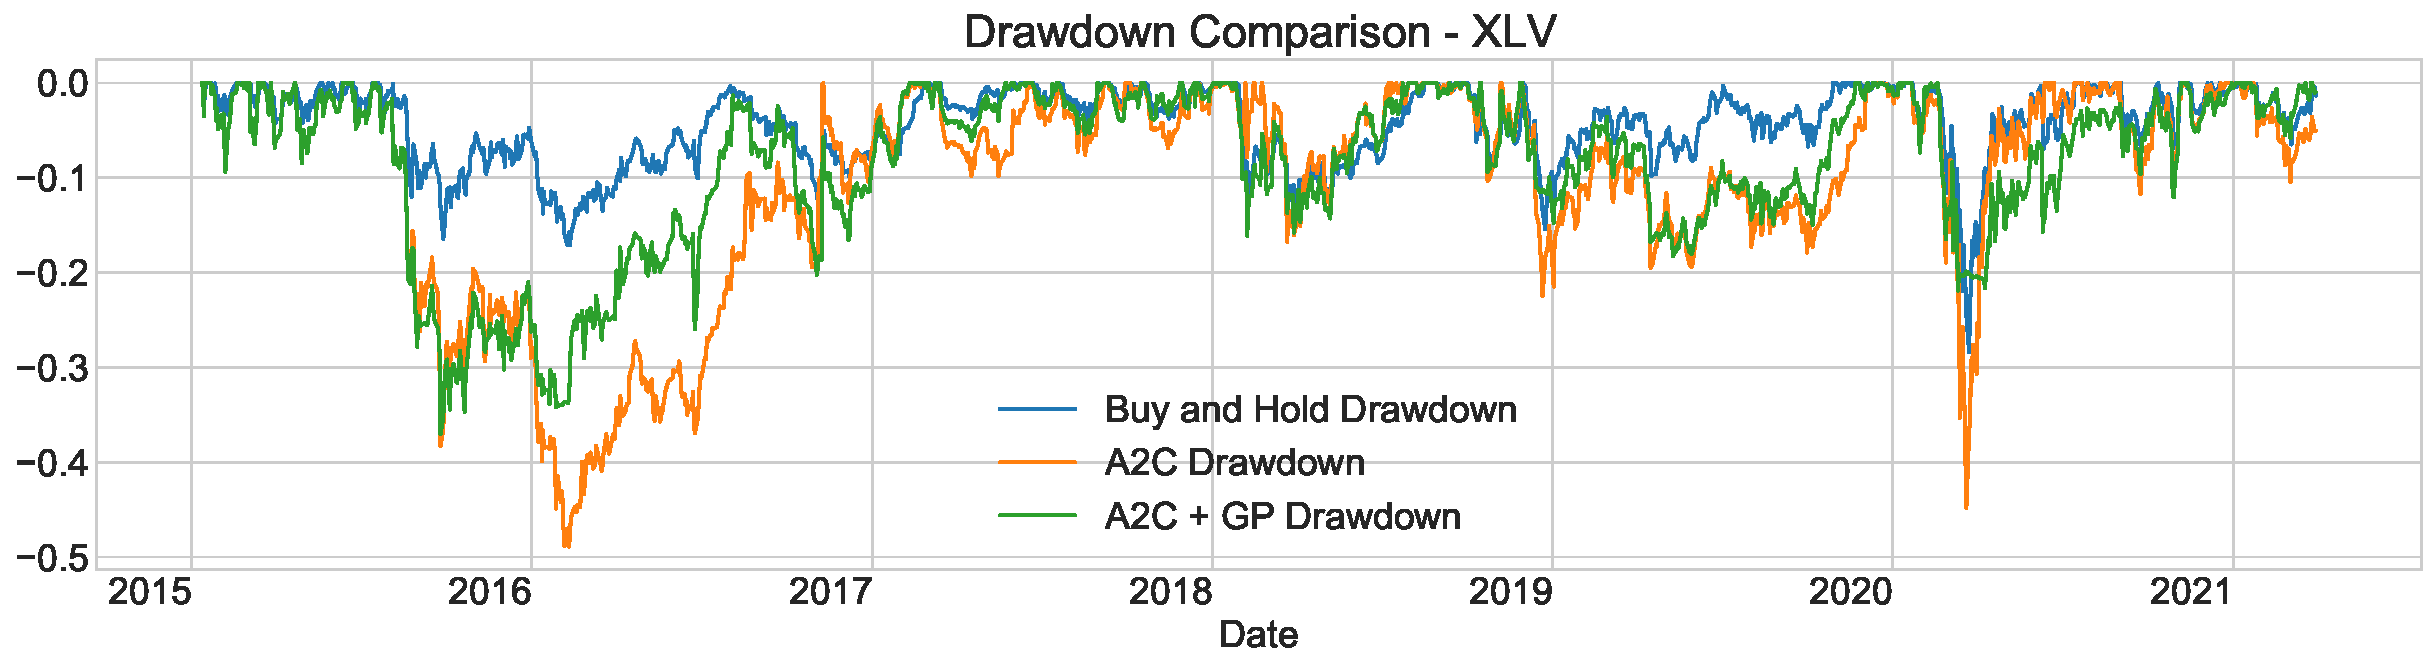
\includegraphics[width=\linewidth]{../src/figures/xlv_drawdowns_comparison.pdf}
	\end{subfigure}
	\caption{}
	\label{fig:xlv}
\end{figure*}

\begin{figure*}[h]
	\centering
	\begin{subfigure}{\linewidth}
		\centering
		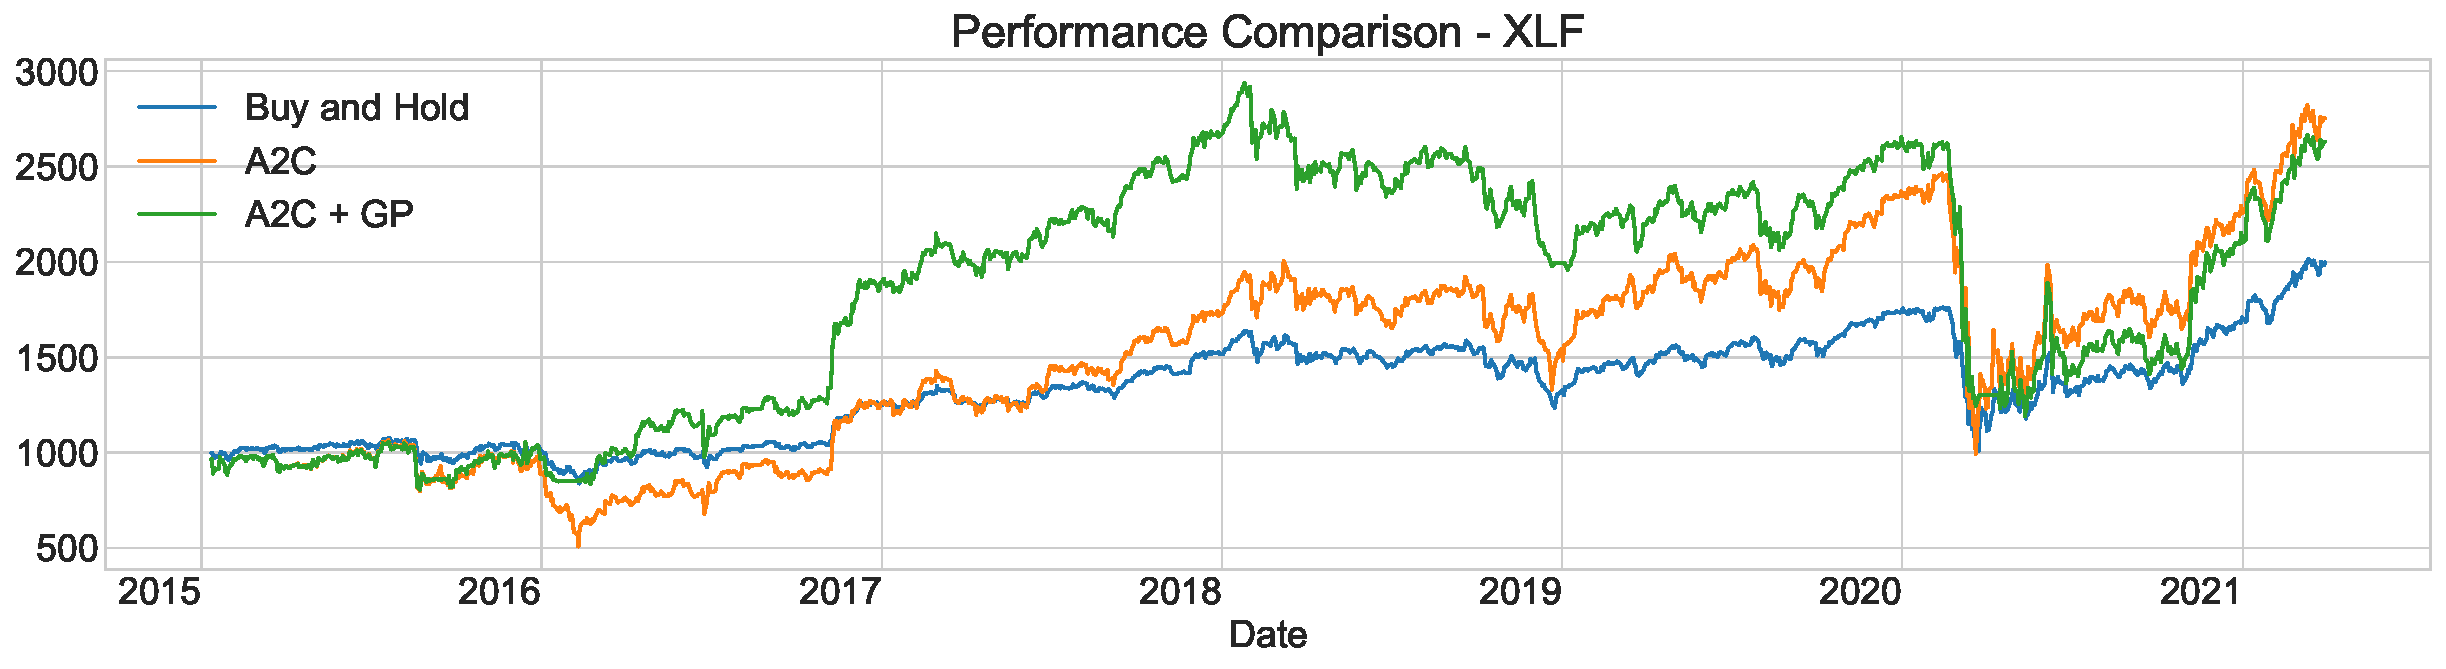
\includegraphics[width=\linewidth]{../src/figures/xlf_performance_comparison.pdf}
	\end{subfigure}
	\begin{subfigure}{\linewidth}
		\centering
		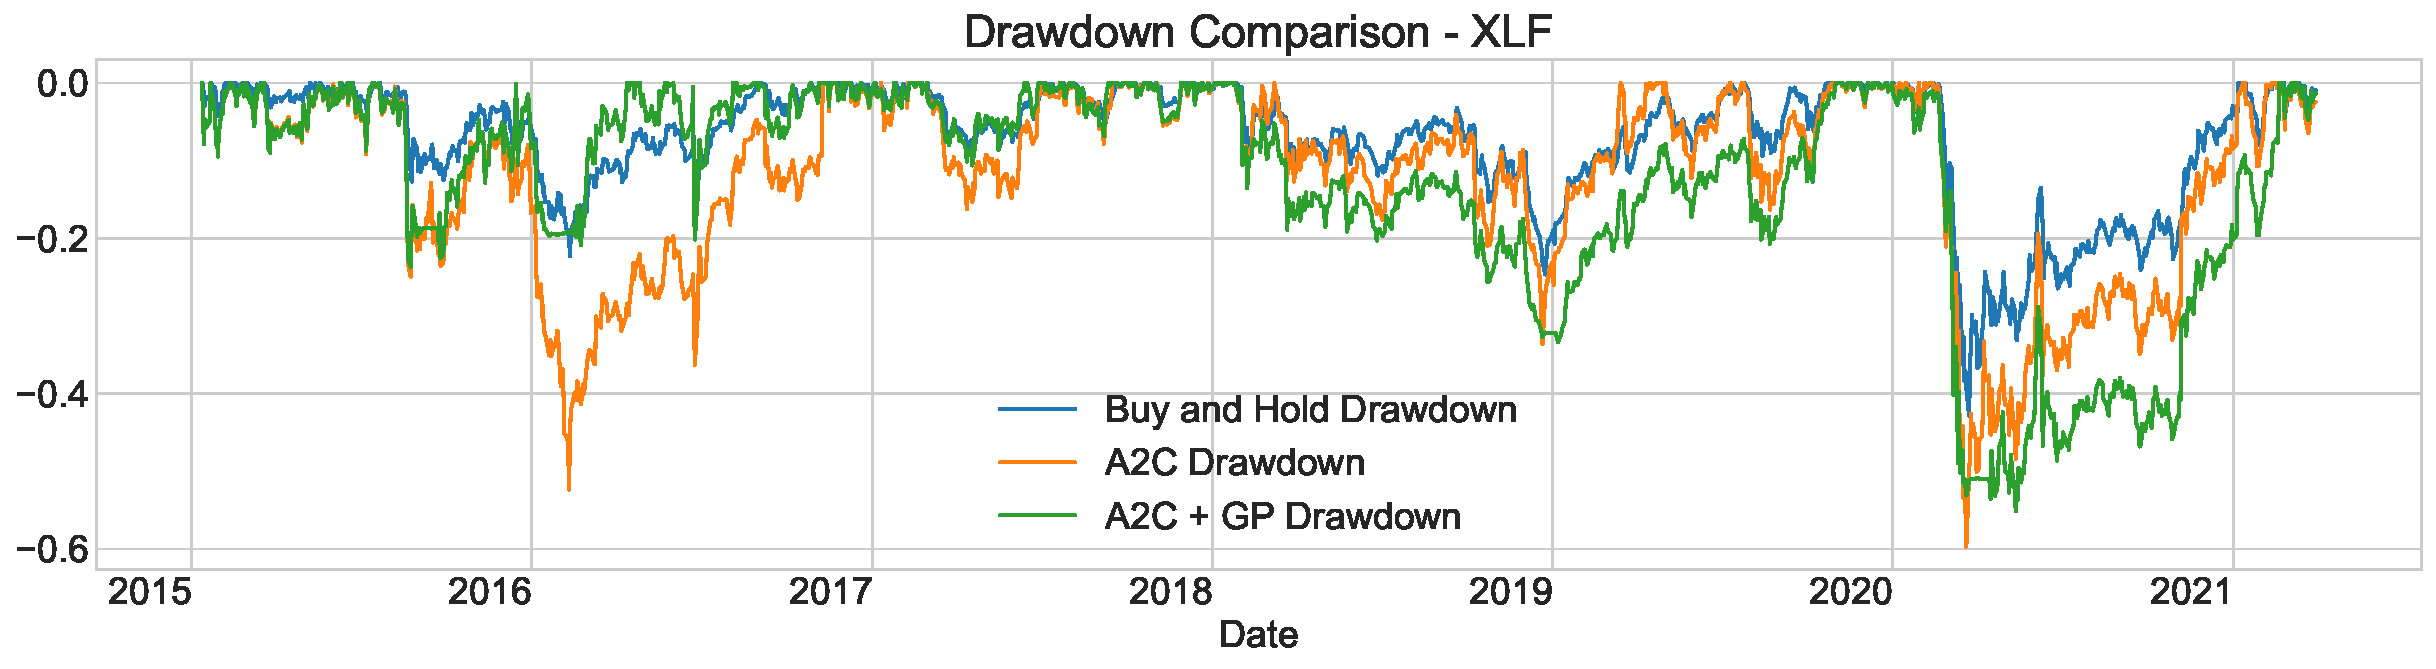
\includegraphics[width=\linewidth]{../src/figures/xlf_drawdowns_comparison.pdf}
	\end{subfigure}
	\caption{}
	\label{fig:xlf}
\end{figure*}

\begin{figure*}[h]
	\centering
	\begin{subfigure}{\linewidth}
		\centering
		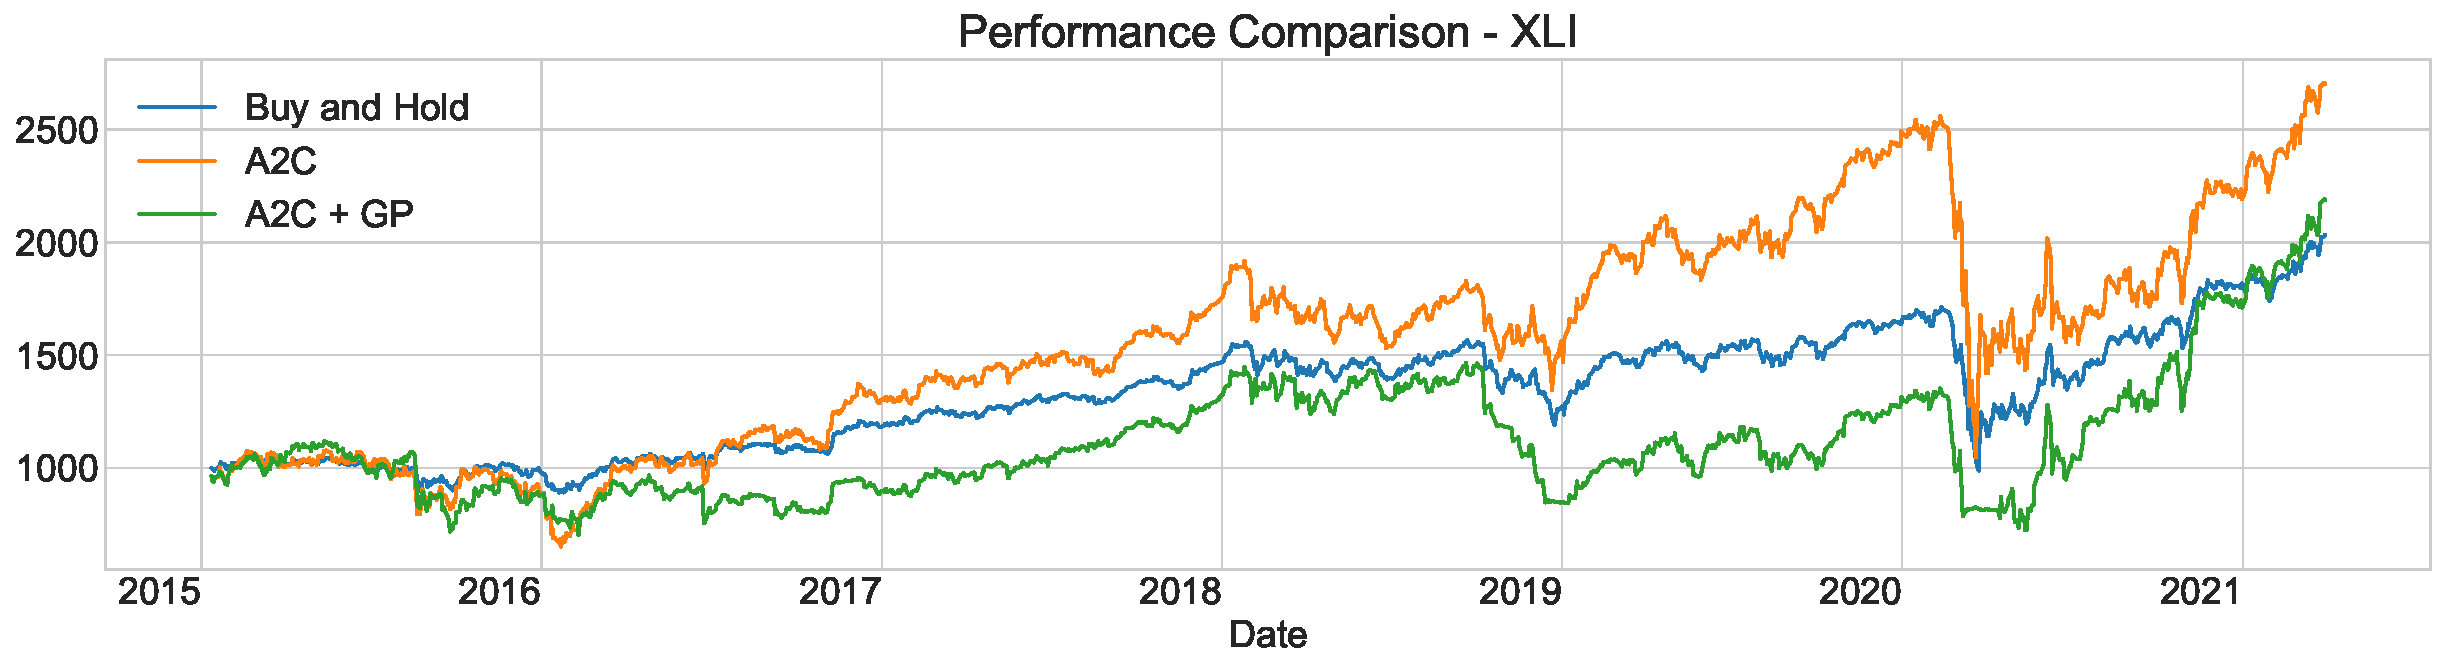
\includegraphics[width=\linewidth]{../src/figures/xli_performance_comparison.pdf}
	\end{subfigure}
	\begin{subfigure}{\linewidth}
		\centering
		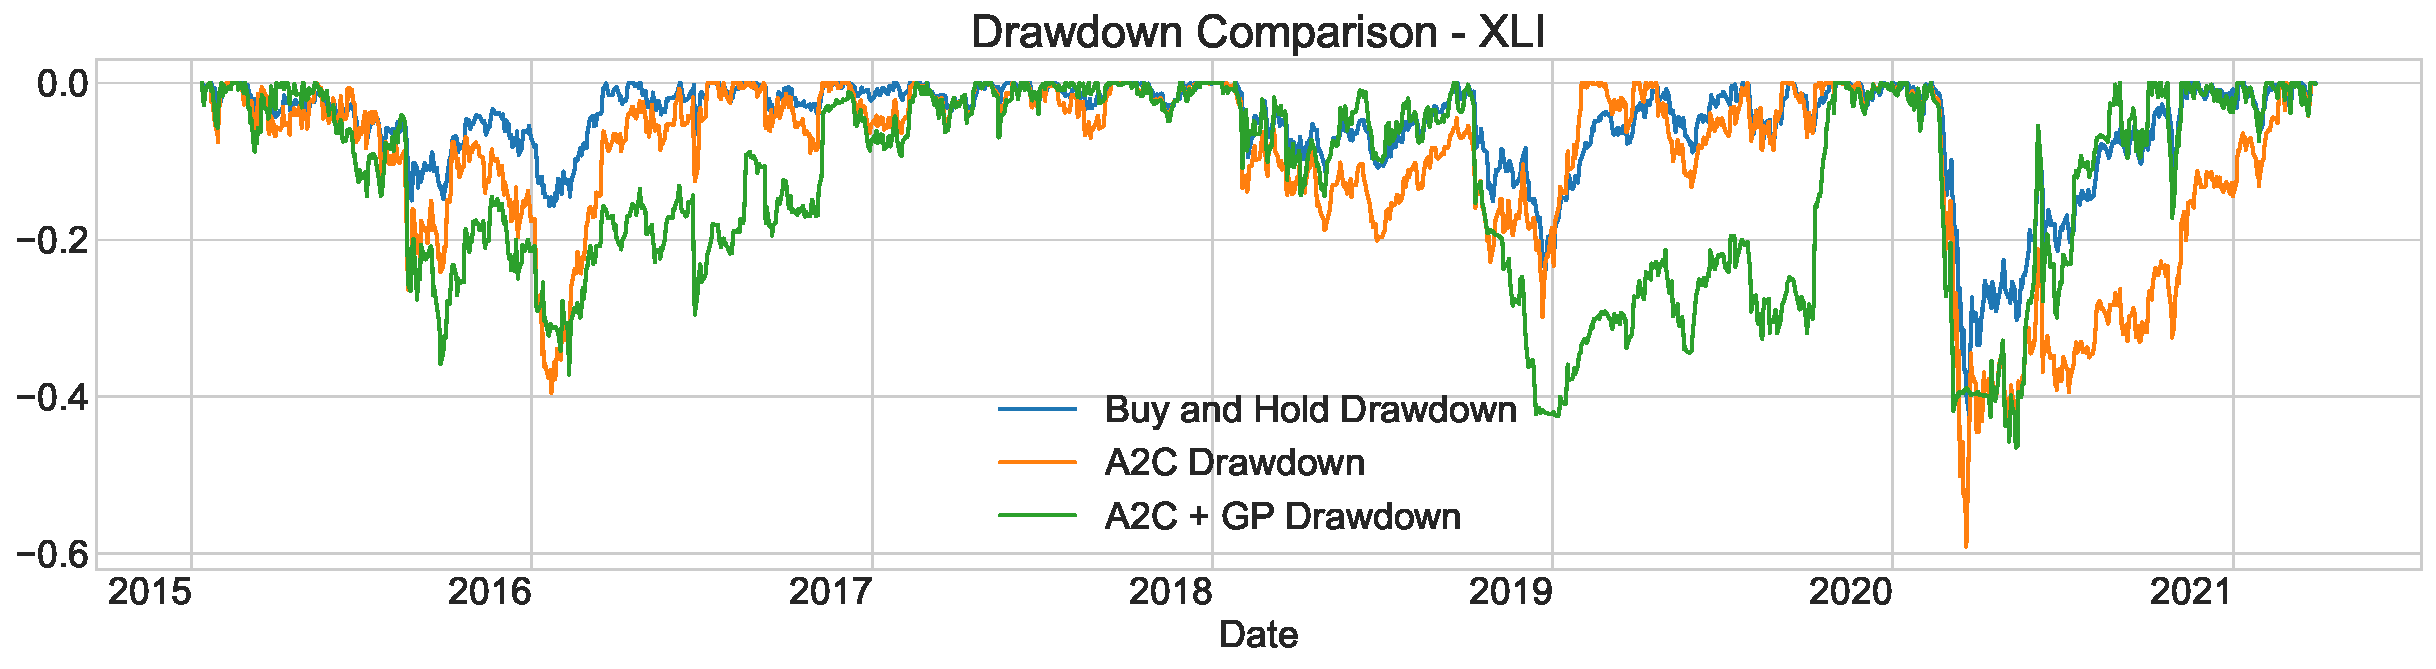
\includegraphics[width=\linewidth]{../src/figures/xli_drawdowns_comparison.pdf}
	\end{subfigure}
	\caption{}
	\label{fig:xli}
\end{figure*}

\begin{figure*}[h]
	\centering
	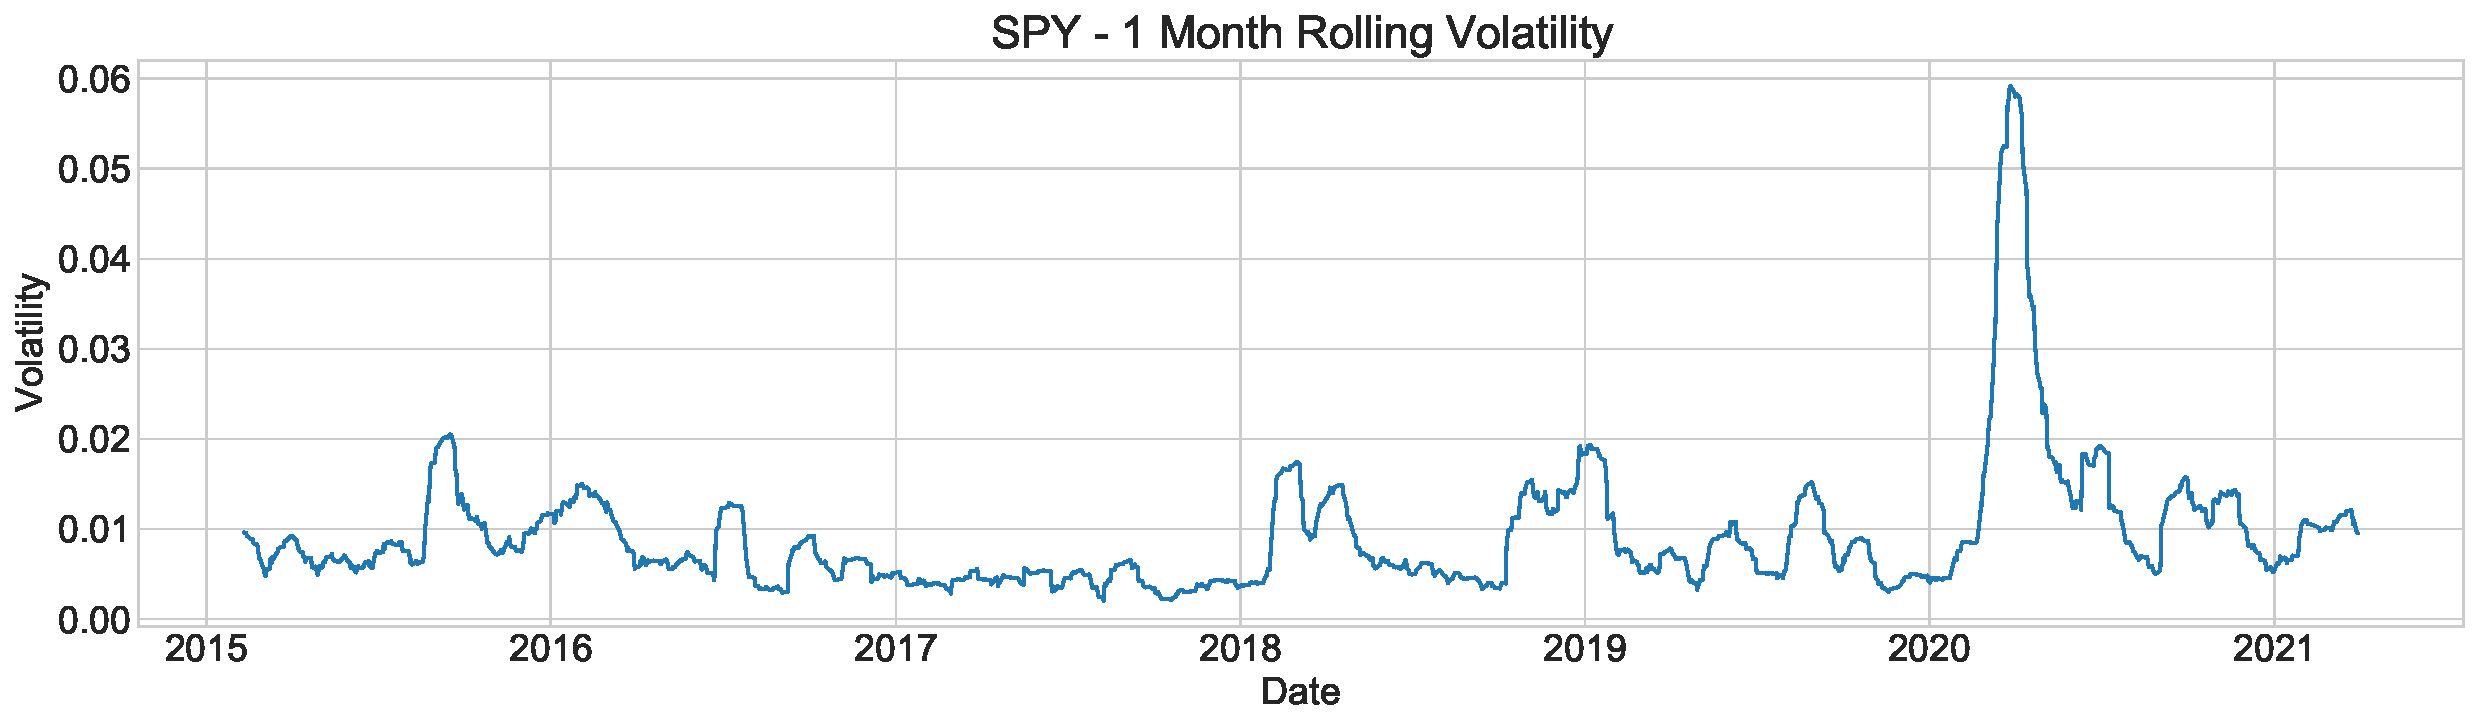
\includegraphics[width=\linewidth]{../src/figures/spy_volatility.pdf}
	\caption{Rolling one-month volatility of the SPY ETF}
	\label{fig:spy vol}
\end{figure*}

\end{document}